\PassOptionsToPackage{unicode=true}{hyperref} % options for packages loaded elsewhere
\PassOptionsToPackage{hyphens}{url}
%
\documentclass[]{book}
\usepackage{lmodern}
\usepackage{amssymb,amsmath}
\usepackage{ifxetex,ifluatex}
\usepackage{fixltx2e} % provides \textsubscript
\ifnum 0\ifxetex 1\fi\ifluatex 1\fi=0 % if pdftex
  \usepackage[T1]{fontenc}
  \usepackage[utf8]{inputenc}
  \usepackage{textcomp} % provides euro and other symbols
\else % if luatex or xelatex
  \usepackage{unicode-math}
  \defaultfontfeatures{Ligatures=TeX,Scale=MatchLowercase}
\fi
% use upquote if available, for straight quotes in verbatim environments
\IfFileExists{upquote.sty}{\usepackage{upquote}}{}
% use microtype if available
\IfFileExists{microtype.sty}{%
\usepackage[]{microtype}
\UseMicrotypeSet[protrusion]{basicmath} % disable protrusion for tt fonts
}{}
\IfFileExists{parskip.sty}{%
\usepackage{parskip}
}{% else
\setlength{\parindent}{0pt}
\setlength{\parskip}{6pt plus 2pt minus 1pt}
}
\usepackage{hyperref}
\hypersetup{
            pdftitle={40 Days and 40 Nights},
            pdfauthor={Martin Morgan; L. Shawn Matott},
            pdfborder={0 0 0},
            breaklinks=true}
\urlstyle{same}  % don't use monospace font for urls
\usepackage{color}
\usepackage{fancyvrb}
\newcommand{\VerbBar}{|}
\newcommand{\VERB}{\Verb[commandchars=\\\{\}]}
\DefineVerbatimEnvironment{Highlighting}{Verbatim}{commandchars=\\\{\}}
% Add ',fontsize=\small' for more characters per line
\usepackage{framed}
\definecolor{shadecolor}{RGB}{248,248,248}
\newenvironment{Shaded}{\begin{snugshade}}{\end{snugshade}}
\newcommand{\AlertTok}[1]{\textcolor[rgb]{0.94,0.16,0.16}{#1}}
\newcommand{\AnnotationTok}[1]{\textcolor[rgb]{0.56,0.35,0.01}{\textbf{\textit{#1}}}}
\newcommand{\AttributeTok}[1]{\textcolor[rgb]{0.77,0.63,0.00}{#1}}
\newcommand{\BaseNTok}[1]{\textcolor[rgb]{0.00,0.00,0.81}{#1}}
\newcommand{\BuiltInTok}[1]{#1}
\newcommand{\CharTok}[1]{\textcolor[rgb]{0.31,0.60,0.02}{#1}}
\newcommand{\CommentTok}[1]{\textcolor[rgb]{0.56,0.35,0.01}{\textit{#1}}}
\newcommand{\CommentVarTok}[1]{\textcolor[rgb]{0.56,0.35,0.01}{\textbf{\textit{#1}}}}
\newcommand{\ConstantTok}[1]{\textcolor[rgb]{0.00,0.00,0.00}{#1}}
\newcommand{\ControlFlowTok}[1]{\textcolor[rgb]{0.13,0.29,0.53}{\textbf{#1}}}
\newcommand{\DataTypeTok}[1]{\textcolor[rgb]{0.13,0.29,0.53}{#1}}
\newcommand{\DecValTok}[1]{\textcolor[rgb]{0.00,0.00,0.81}{#1}}
\newcommand{\DocumentationTok}[1]{\textcolor[rgb]{0.56,0.35,0.01}{\textbf{\textit{#1}}}}
\newcommand{\ErrorTok}[1]{\textcolor[rgb]{0.64,0.00,0.00}{\textbf{#1}}}
\newcommand{\ExtensionTok}[1]{#1}
\newcommand{\FloatTok}[1]{\textcolor[rgb]{0.00,0.00,0.81}{#1}}
\newcommand{\FunctionTok}[1]{\textcolor[rgb]{0.00,0.00,0.00}{#1}}
\newcommand{\ImportTok}[1]{#1}
\newcommand{\InformationTok}[1]{\textcolor[rgb]{0.56,0.35,0.01}{\textbf{\textit{#1}}}}
\newcommand{\KeywordTok}[1]{\textcolor[rgb]{0.13,0.29,0.53}{\textbf{#1}}}
\newcommand{\NormalTok}[1]{#1}
\newcommand{\OperatorTok}[1]{\textcolor[rgb]{0.81,0.36,0.00}{\textbf{#1}}}
\newcommand{\OtherTok}[1]{\textcolor[rgb]{0.56,0.35,0.01}{#1}}
\newcommand{\PreprocessorTok}[1]{\textcolor[rgb]{0.56,0.35,0.01}{\textit{#1}}}
\newcommand{\RegionMarkerTok}[1]{#1}
\newcommand{\SpecialCharTok}[1]{\textcolor[rgb]{0.00,0.00,0.00}{#1}}
\newcommand{\SpecialStringTok}[1]{\textcolor[rgb]{0.31,0.60,0.02}{#1}}
\newcommand{\StringTok}[1]{\textcolor[rgb]{0.31,0.60,0.02}{#1}}
\newcommand{\VariableTok}[1]{\textcolor[rgb]{0.00,0.00,0.00}{#1}}
\newcommand{\VerbatimStringTok}[1]{\textcolor[rgb]{0.31,0.60,0.02}{#1}}
\newcommand{\WarningTok}[1]{\textcolor[rgb]{0.56,0.35,0.01}{\textbf{\textit{#1}}}}
\usepackage{longtable,booktabs}
% Fix footnotes in tables (requires footnote package)
\IfFileExists{footnote.sty}{\usepackage{footnote}\makesavenoteenv{longtable}}{}
\usepackage{graphicx,grffile}
\makeatletter
\def\maxwidth{\ifdim\Gin@nat@width>\linewidth\linewidth\else\Gin@nat@width\fi}
\def\maxheight{\ifdim\Gin@nat@height>\textheight\textheight\else\Gin@nat@height\fi}
\makeatother
% Scale images if necessary, so that they will not overflow the page
% margins by default, and it is still possible to overwrite the defaults
% using explicit options in \includegraphics[width, height, ...]{}
\setkeys{Gin}{width=\maxwidth,height=\maxheight,keepaspectratio}
\setlength{\emergencystretch}{3em}  % prevent overfull lines
\providecommand{\tightlist}{%
  \setlength{\itemsep}{0pt}\setlength{\parskip}{0pt}}
\setcounter{secnumdepth}{5}
% Redefines (sub)paragraphs to behave more like sections
\ifx\paragraph\undefined\else
\let\oldparagraph\paragraph
\renewcommand{\paragraph}[1]{\oldparagraph{#1}\mbox{}}
\fi
\ifx\subparagraph\undefined\else
\let\oldsubparagraph\subparagraph
\renewcommand{\subparagraph}[1]{\oldsubparagraph{#1}\mbox{}}
\fi

% set default figure placement to htbp
\makeatletter
\def\fps@figure{htbp}
\makeatother

\usepackage{booktabs}
\usepackage[]{natbib}
\bibliographystyle{apalike}

\title{40 Days and 40 Nights}
\author{Martin Morgan \and L. Shawn Matott}
\date{2020-04-15}

\begin{document}
\maketitle

{
\setcounter{tocdepth}{1}
\tableofcontents
}
\hypertarget{motivation}{%
\chapter*{Motivation}\label{motivation}}
\addcontentsline{toc}{chapter}{Motivation}

This is a WORK IN PROGRESS.

This course was suggested and enabled by Adam Kisailus and Richard Hershberger. It is available for Roswell Park graduate students.

\hypertarget{introduction}{%
\section*{Introduction}\label{introduction}}
\addcontentsline{toc}{section}{Introduction}

The word `\href{https://www.etymonline.com/word/quarantine}{quarantine}' is from the 1660's and refers to the fourty days (Italian \emph{quaranta giorni}) a ship suspected of carrying disease was kept in isolation.

What to do in a quarantine? The astronaut Scott Kelly spent nearly a year on the International Space Station. In a New York Times \href{https://www.nytimes.com/2020/03/21/opinion/scott-kelly-coronavirus-isolation.html}{opinion piece} he says, among other things, that `you need a hobby', and what better hobby than a useful one? Let's take the opportunity provided by COVID-19 to learn R for statistical analysis and comprehension of data. Who knows, it may be useful after all this is over!

\hypertarget{what-to-expect}{%
\section*{What to expect}\label{what-to-expect}}
\addcontentsline{toc}{section}{What to expect}

We'll meet via zoom twice a week, Mondays and Fridays, for one hour. We'll use this time to make sure everyone is making progress, and to introduce new or more difficult topics. Other days we'll have short exercises and activities that hopefully provide an opportunity to learn at your own speed.

We haven't thought this through much, but roughly we might cover:

\begin{itemize}
\item
  Week \ref{one}: We'll start with the basics of installing and using R. We'll set up \emph{R} and \emph{RStudio} on your local computer, or if that doesn't work use a cloud-based RStudio. We'll learn the basics of \emph{R} -- numeric, character, logical, and other vectors; variables; and slightly more complicated representations of `factors' and dates. We'll also use \emph{RStudio} to write a script that allows us to easily re-create an analysis, illustrating the power concept of \emph{reproducible research}.

\begin{Shaded}
\begin{Highlighting}[]
\NormalTok{activity <-}\StringTok{ }\KeywordTok{c}\NormalTok{(}\StringTok{"check e-mail"}\NormalTok{, }\StringTok{"breakfast"}\NormalTok{, }\StringTok{"conference call"}\NormalTok{, }\StringTok{"webinar"}\NormalTok{, }\StringTok{"walk"}\NormalTok{)}
\NormalTok{minutes_per_activity <-}\StringTok{ }\KeywordTok{c}\NormalTok{(}\DecValTok{20}\NormalTok{, }\DecValTok{30}\NormalTok{, }\DecValTok{60}\NormalTok{, }\DecValTok{60}\NormalTok{, }\DecValTok{60}\NormalTok{)}
\NormalTok{minutes_per_activity }\OperatorTok{>=}\StringTok{ }\DecValTok{60}
\CommentTok{## [1] FALSE FALSE  TRUE  TRUE  TRUE}
\NormalTok{activity[minutes_per_activity }\OperatorTok{>=}\StringTok{ }\DecValTok{60}\NormalTok{]}
\CommentTok{## [1] "conference call" "webinar"         "walk"}
\end{Highlighting}
\end{Shaded}
\item
  Week \ref{two}: The \texttt{data.frame}. This week is all about \emph{R}'s \texttt{data.frame}, a versatile way of representing and manipulating a table (like an Excel spreadsheet) of data. We'll learn how to create, write, and read a \texttt{data.frame}; how to go from data in a spreadsheet in Excel to a \texttt{data.frame} in \emph{R}; and how to perform simple manipulations on a \texttt{data.frame}, like creating a subset of data, summarizing values in a column, and summarizing values in one column based on a grouping variable in another column.

\begin{Shaded}
\begin{Highlighting}[]
\NormalTok{url =}\StringTok{ "https://raw.githubusercontent.com/nytimes/covid-19-data/master/us-counties.csv"}
\NormalTok{cases <-}\StringTok{ }\KeywordTok{read.csv}\NormalTok{(url)}
\NormalTok{erie <-}\StringTok{ }\KeywordTok{subset}\NormalTok{(cases, county }\OperatorTok{==}\StringTok{ "Erie"} \OperatorTok{&}\StringTok{ }\NormalTok{state }\OperatorTok{==}\StringTok{ "New York"}\NormalTok{)}
\KeywordTok{tail}\NormalTok{(erie)}
\CommentTok{##             date county    state  fips cases deaths}
\CommentTok{## 44803 2020-04-09   Erie New York 36029  1362     46}
\CommentTok{## 47417 2020-04-10   Erie New York 36029  1409     58}
\CommentTok{## 50071 2020-04-11   Erie New York 36029  1472     62}
\CommentTok{## 52744 2020-04-12   Erie New York 36029  1571     75}
\CommentTok{## 55428 2020-04-13   Erie New York 36029  1624     86}
\CommentTok{## 58128 2020-04-14   Erie New York 36029  1668     99}
\end{Highlighting}
\end{Shaded}
\item
  Week \ref{three}: Packages for extending \emph{R}. A great strength of \emph{R} is its extensibility through packages. We'll learn about \href{https://cran.r-project.org}{CRAN}, and install and use the `tidyverse' suite of packages. The tidyverse provides us with an alternative set of tools for working with tabular data, and We'll use publicly available data to explore the spread of COVID-19 in the US. We'll read, filter, mutate (change), and select subsets of the data, and group data by one column (e.g., `state') to create summaries (e.g., cases per state). We'll also start to explore data visualization, creating our first plots of the spread of COVID-19.

\begin{Shaded}
\begin{Highlighting}[]
\KeywordTok{library}\NormalTok{(dplyr)}
\KeywordTok{library}\NormalTok{(ggplot2)}
\CommentTok{## ...additional commands}
\end{Highlighting}
\end{Shaded}

  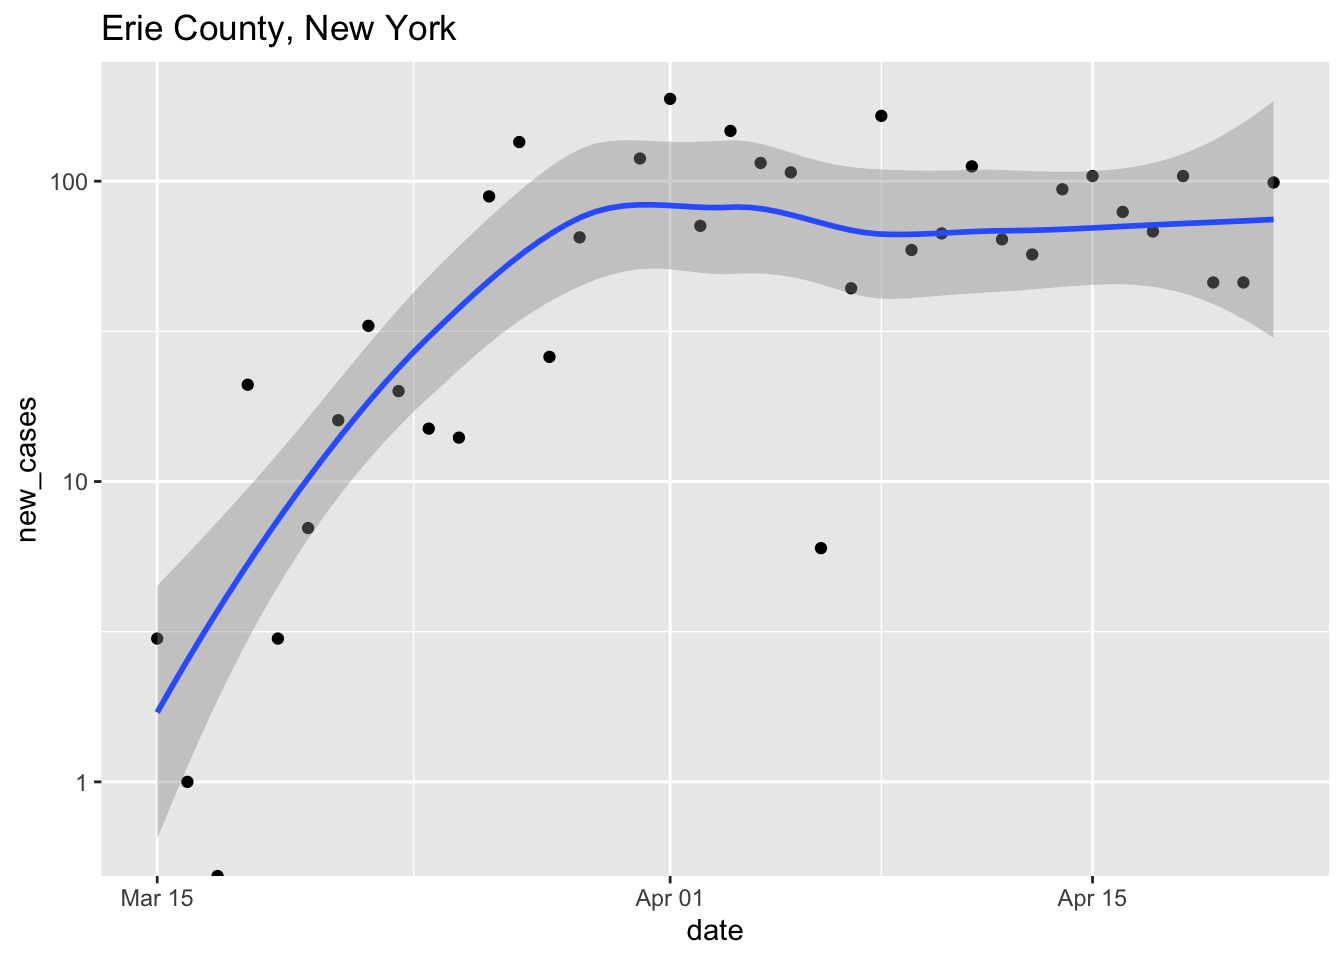
\includegraphics{index_files/figure-latex/unnamed-chunk-4-1.pdf}
\item
  Week \ref{four}: Maps. This week will be a specialized topic, tackling relatively advanced challenges associated with spatial visualization.
\item
  Week \ref{five}: Bioinformatic analysis with \href{https://bioconductor.org}{Bioconductor}. \emph{Bioconductor} is a collection of more than 1800 \emph{R} packages for the statistical analysis and comprehension of high-throughput genomic data. We'll use \emph{Bioconductor} to look at COVID-19 genome sequences, and to explore emerging genomic data relevant to the virus.
\item
  Week \ref{six}: COVID-19 has really shown the value of open data and collaboration. In the final week of our quarantine, we'll explore collaboration; developing independent and group projects that synthesize the use of \emph{R} to explore data. We'll learn tools of collaboration including git and github, and develop `best practices' for robust, reproducible research. We'll learn about writing `markdown' reports to share our project with others.
\end{itemize}

\hypertarget{one}{%
\chapter{Basics}\label{one}}

\hypertarget{day-1-monday-zoom-orientation}{%
\section{Day 1 (Monday) Zoom orientation}\label{day-1-monday-zoom-orientation}}

\hypertarget{logistics-10-minutes}{%
\subsection{Logistics (10 minutes)}\label{logistics-10-minutes}}

Course material

\begin{itemize}
\tightlist
\item
  Available at \url{https://mtmorgan.github.io/QuaRantine}
\end{itemize}

Cadence

\begin{itemize}
\tightlist
\item
  Monday and Friday group zoom sessions -- these will review and troubleshoot previous material, and outline goals for the next set of independent activities.
\item
  Daily independent activities -- most of your learning will happen here!
\end{itemize}

Communicating

\begin{itemize}
\tightlist
\item
  We'll use Microsoft Teams (if most participants have access to the course)
\item
  Visit Microsoft \href{https://teams.microsoft.org}{teams} and sign in with your Roswell username (e.g., \texttt{MA38727@RoswellPark.org}) and the password you use to check email, etc. Join the `QuaRantine' team.
\end{itemize}

\hypertarget{installing-r-and-rstudio-25-minutes-shawn}{%
\subsection{\texorpdfstring{Installing \emph{R} and \emph{RStudio} (25 minutes, Shawn)}{Installing R and RStudio (25 minutes, Shawn)}}\label{installing-r-and-rstudio-25-minutes-shawn}}

What is R?

\begin{itemize}
\item
  A programming language for statistical computing, data analysis and scientific graphics.
\item
  Open-source with a large (and growing) user community.
\item
  Currently in the top 10 most popular languages according to the \href{https://www.tiobe.com/tiobe-index/}{tiobe index}.
\end{itemize}

What is \href{https://rstudio.com/}{RStudio}?

\begin{itemize}
\tightlist
\item
  RStudio provides an integrated editor and shell environment to make R programming easier. Some of the more useful features include:

  \begin{itemize}
  \tightlist
  \item
    Syntax highlighting and color coding
  \item
    Easy switching between shell and editor
  \item
    Dynamic help and docs
  \end{itemize}
\end{itemize}

Installing \emph{R} and \emph{RStudio}

\begin{itemize}
\tightlist
\item
  Two ways to ``get'' RStudio:

  \begin{itemize}
  \tightlist
  \item
    Install on your laptop or desktop

    \begin{itemize}
    \tightlist
    \item
      Download the free desktop \href{https://rstudio.com/products/rstudio/download/\#download}{installer here}
    \end{itemize}
  \item
    Use the rstudio.cloud resource

    \begin{itemize}
    \tightlist
    \item
      \href{https://rstudio.cloud/}{Visit rstudio.cloud}, sign-up, and sign-on
    \end{itemize}
  \end{itemize}
\end{itemize}

The preferred approach for this course is to try to install R and RStudio on your own computer

\begin{itemize}
\tightlist
\item
  Windows Users:

  \begin{itemize}
  \tightlist
  \item
    \href{https://cran.rstudio.com/bin/windows/base/R-3.6.3-win.exe}{Download R for Windows} and run the installer. Avoid, if possible, installing as administrator.
  \item
    \href{https://download1.rstudio.org/desktop/windows/RStudio-1.2.5033.exe}{Download RStudio for Windows} and run the installer.
  \item
    Test the installation by launching RStudio. You should end up with a window like the screen shot below.
  \end{itemize}
\item
  Mac Users:

  \begin{itemize}
  \tightlist
  \item
    \href{https://cran.rstudio.com/bin/macosx/R-3.6.3.pkg}{Download R for macOS} (OS X 10.11, El Capitan, and later) or \href{https://cran.rstudio.com/bin/macosx/R-3.6.3.nn.pkg}{older macOS} and run the installer.
  \item
    \href{https://download1.rstudio.org/desktop/macos/RStudio-1.2.5033.dmg}{Download RStudio for macOS} and run the installer.
  \item
    Test the installation by launching RStudio. You should end up with a window like the screen shot below.
  \end{itemize}
\end{itemize}

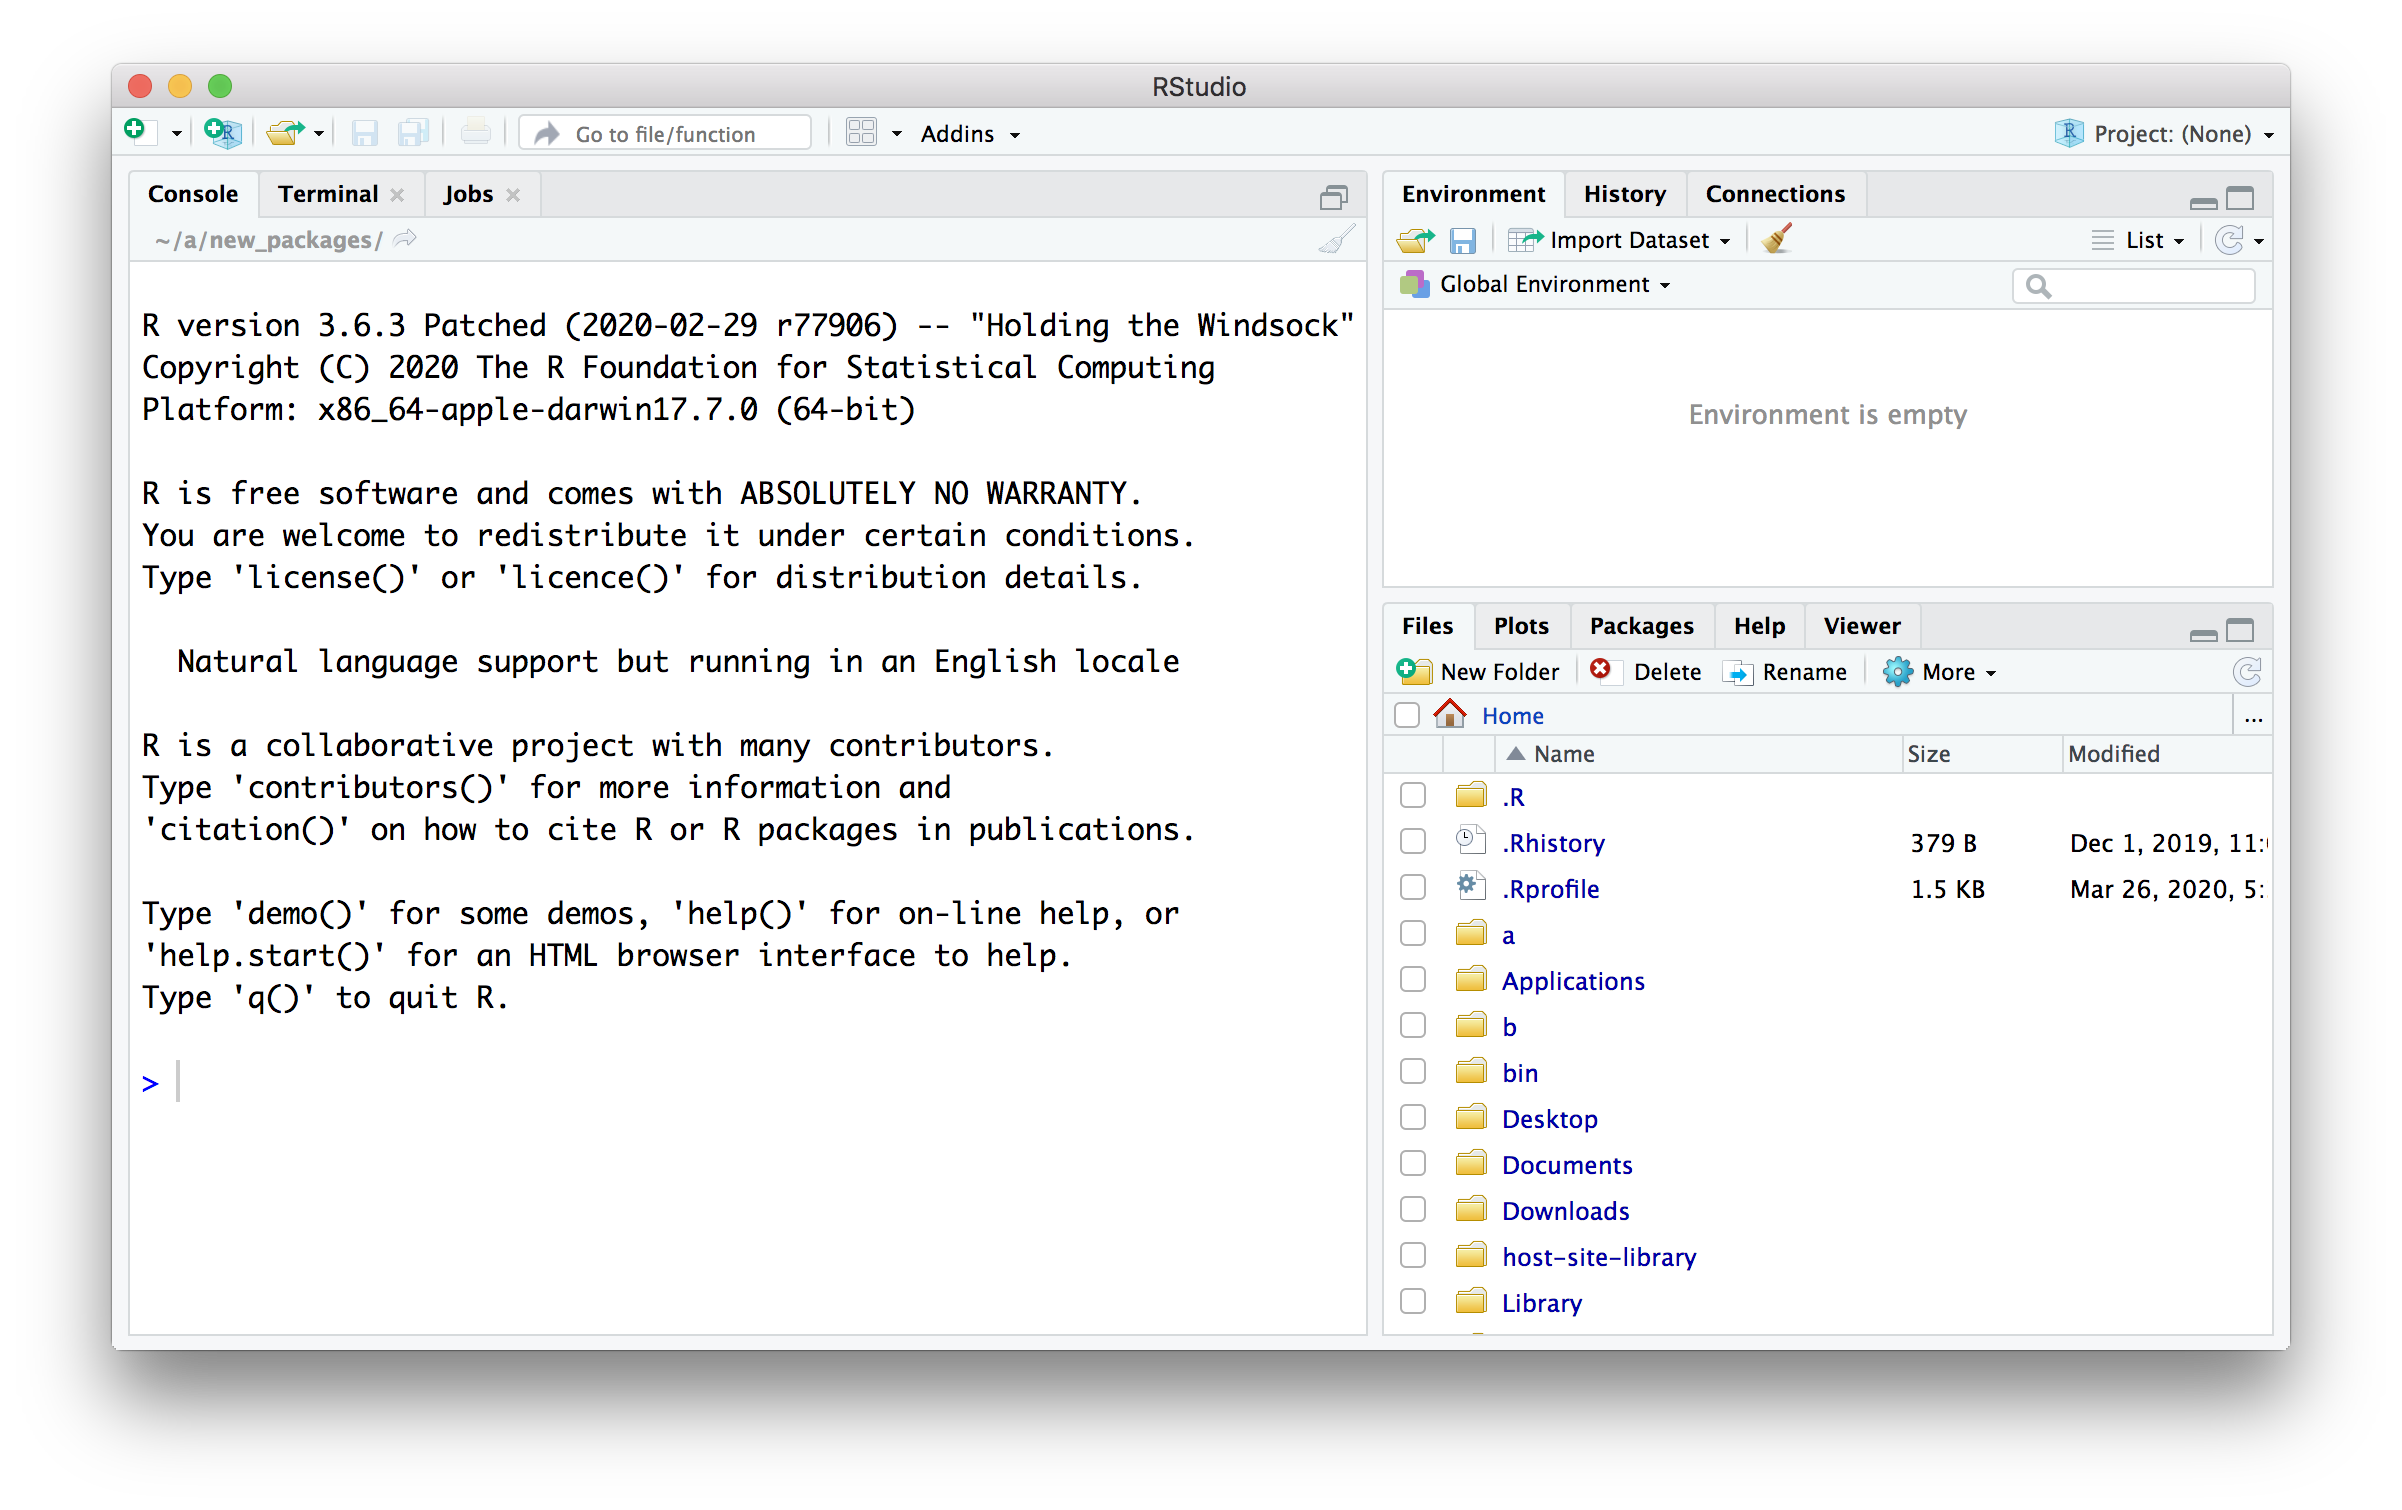
\includegraphics[width=33.36in]{images/RStudio-screenshot}

An ALTERNATIVE, if installing on your own computer does not work:

\begin{itemize}
\item
  Do the following only if you are NOT ABLE TO INSTALL R and RStudio.
\item
  Visit \href{https://rstudio.cloud/}{rstudio.cloud}. Click the `Get Started' button, and create an account (I used my gmail account\ldots{}). You should end up at a screen like the following.

  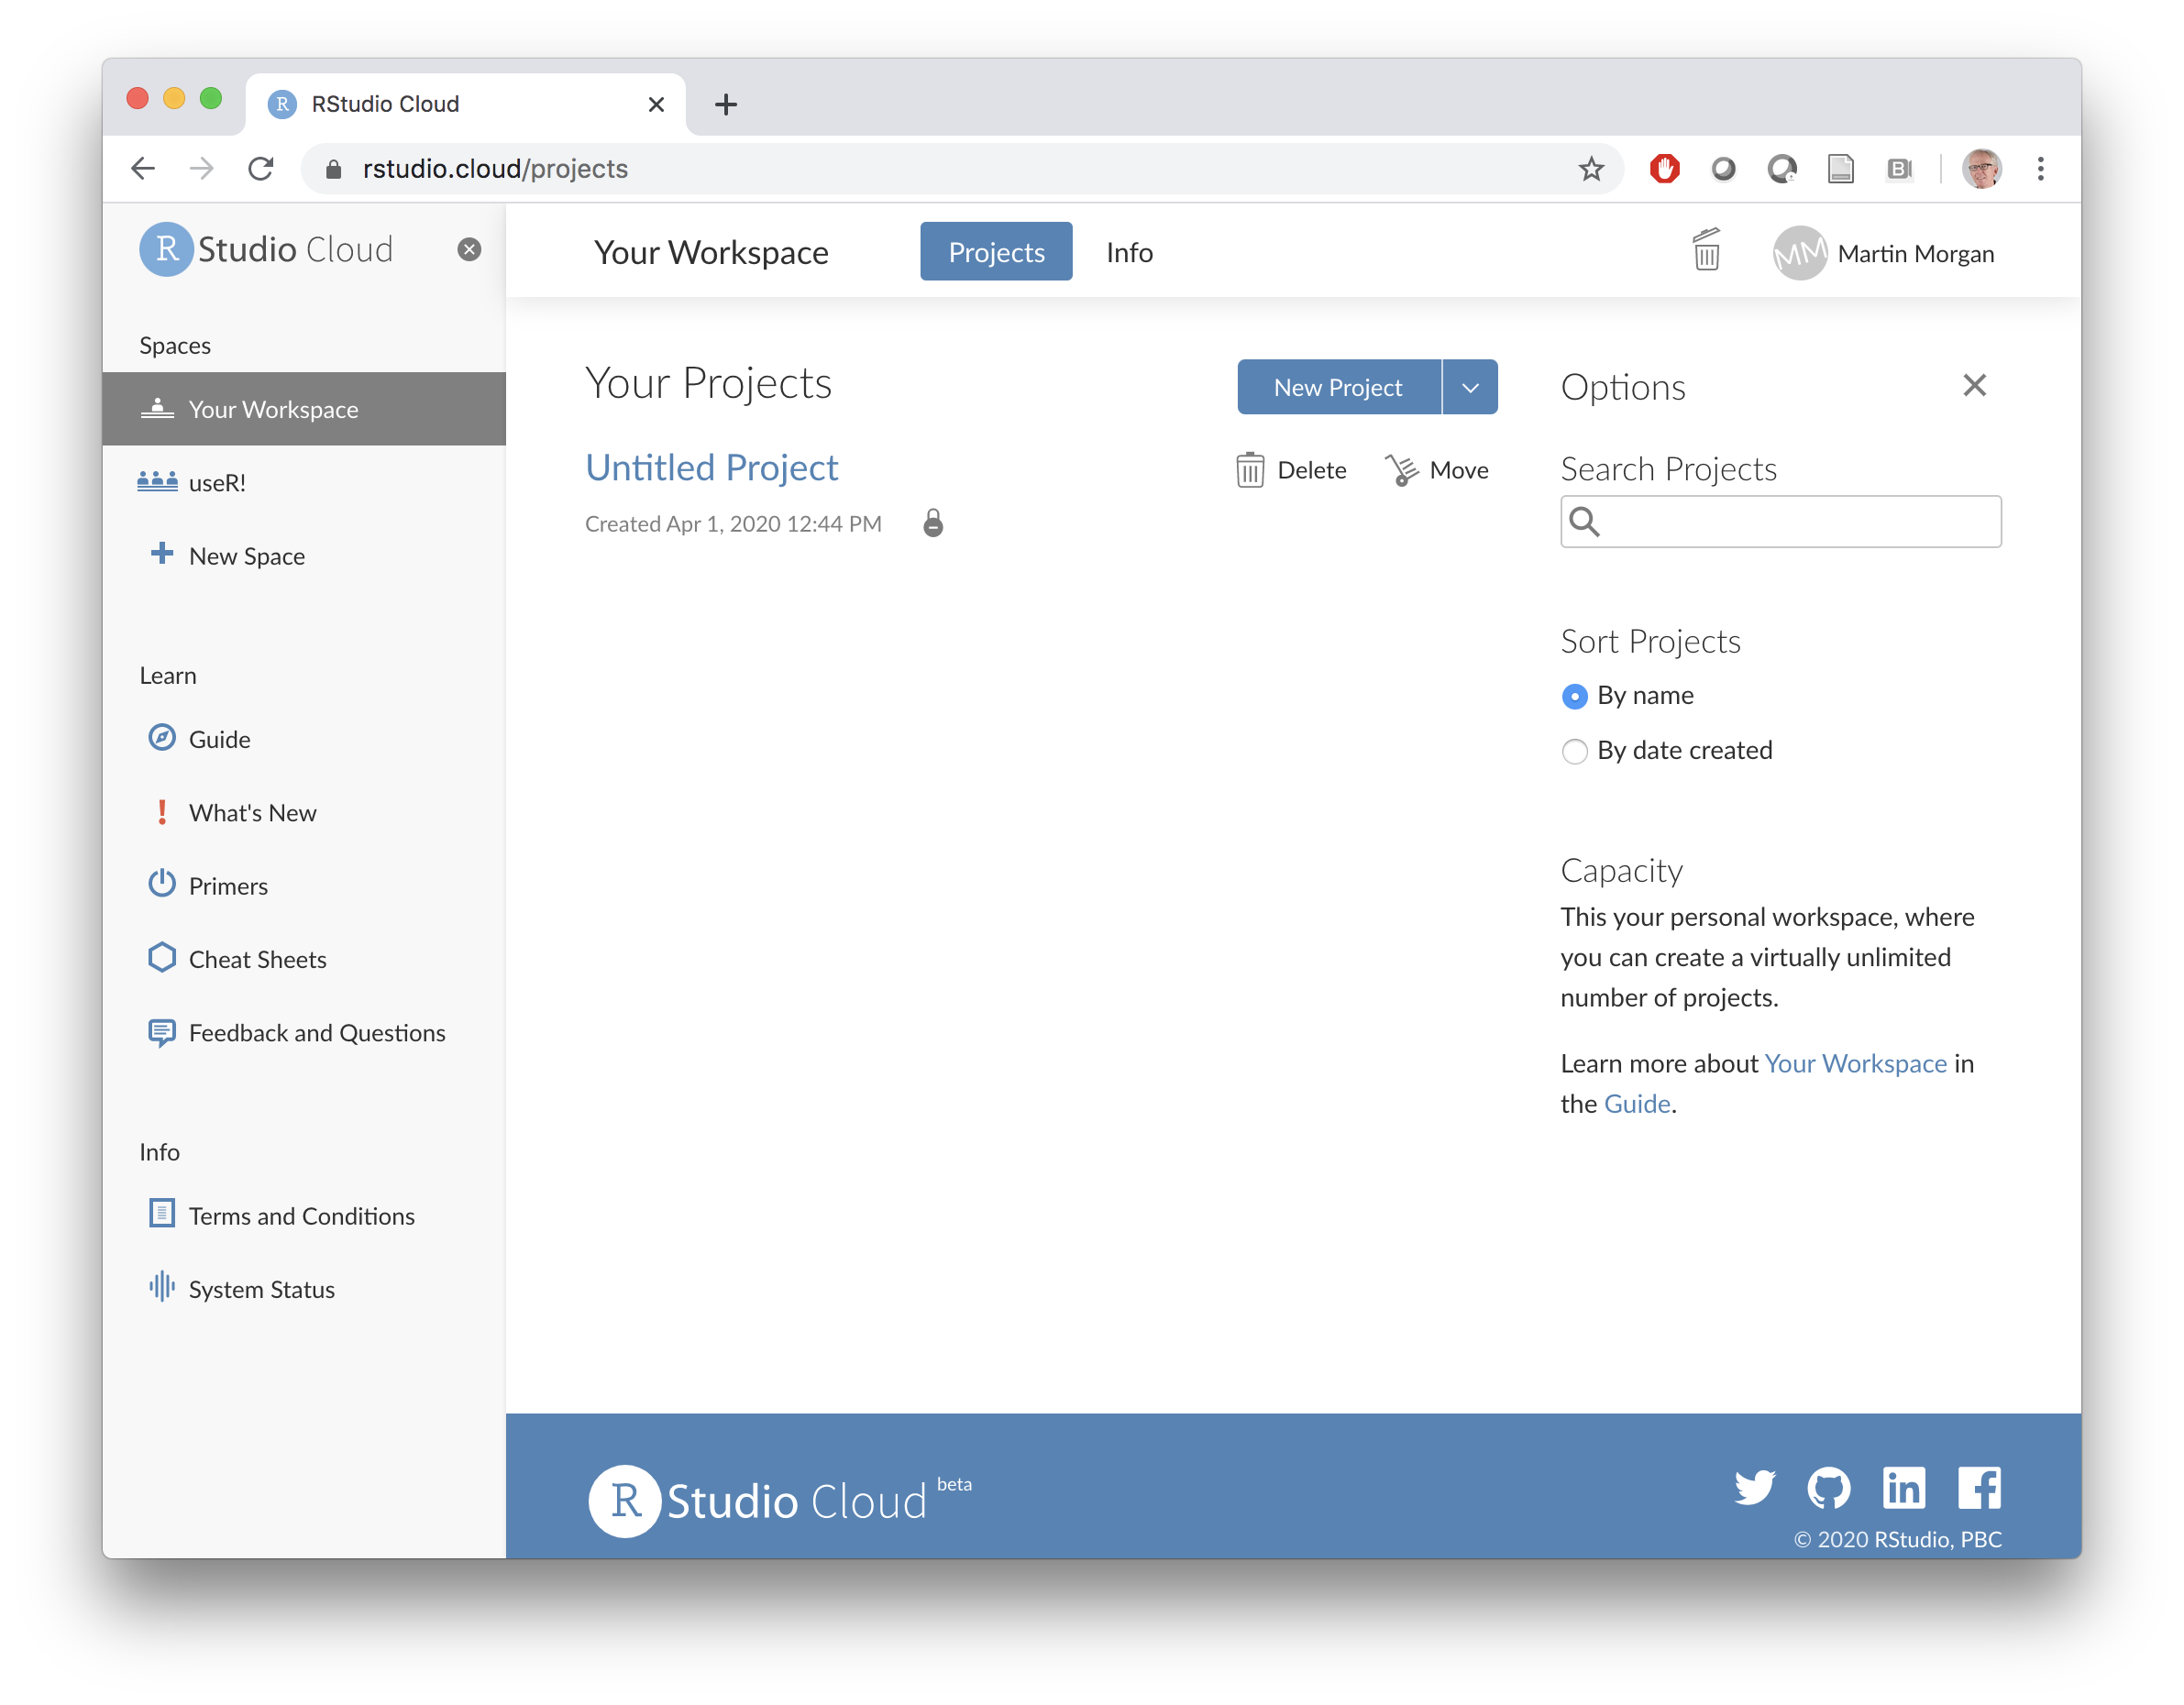
\includegraphics[width=33.08in]{images/RStudio-cloud-screenshot}
\item
  Click on the `New Project' button, to end up with a screen like the one below. Note the `Untitled Project' at the top of the screen; click on it to name your project, e.g., `QuaRantine'.

  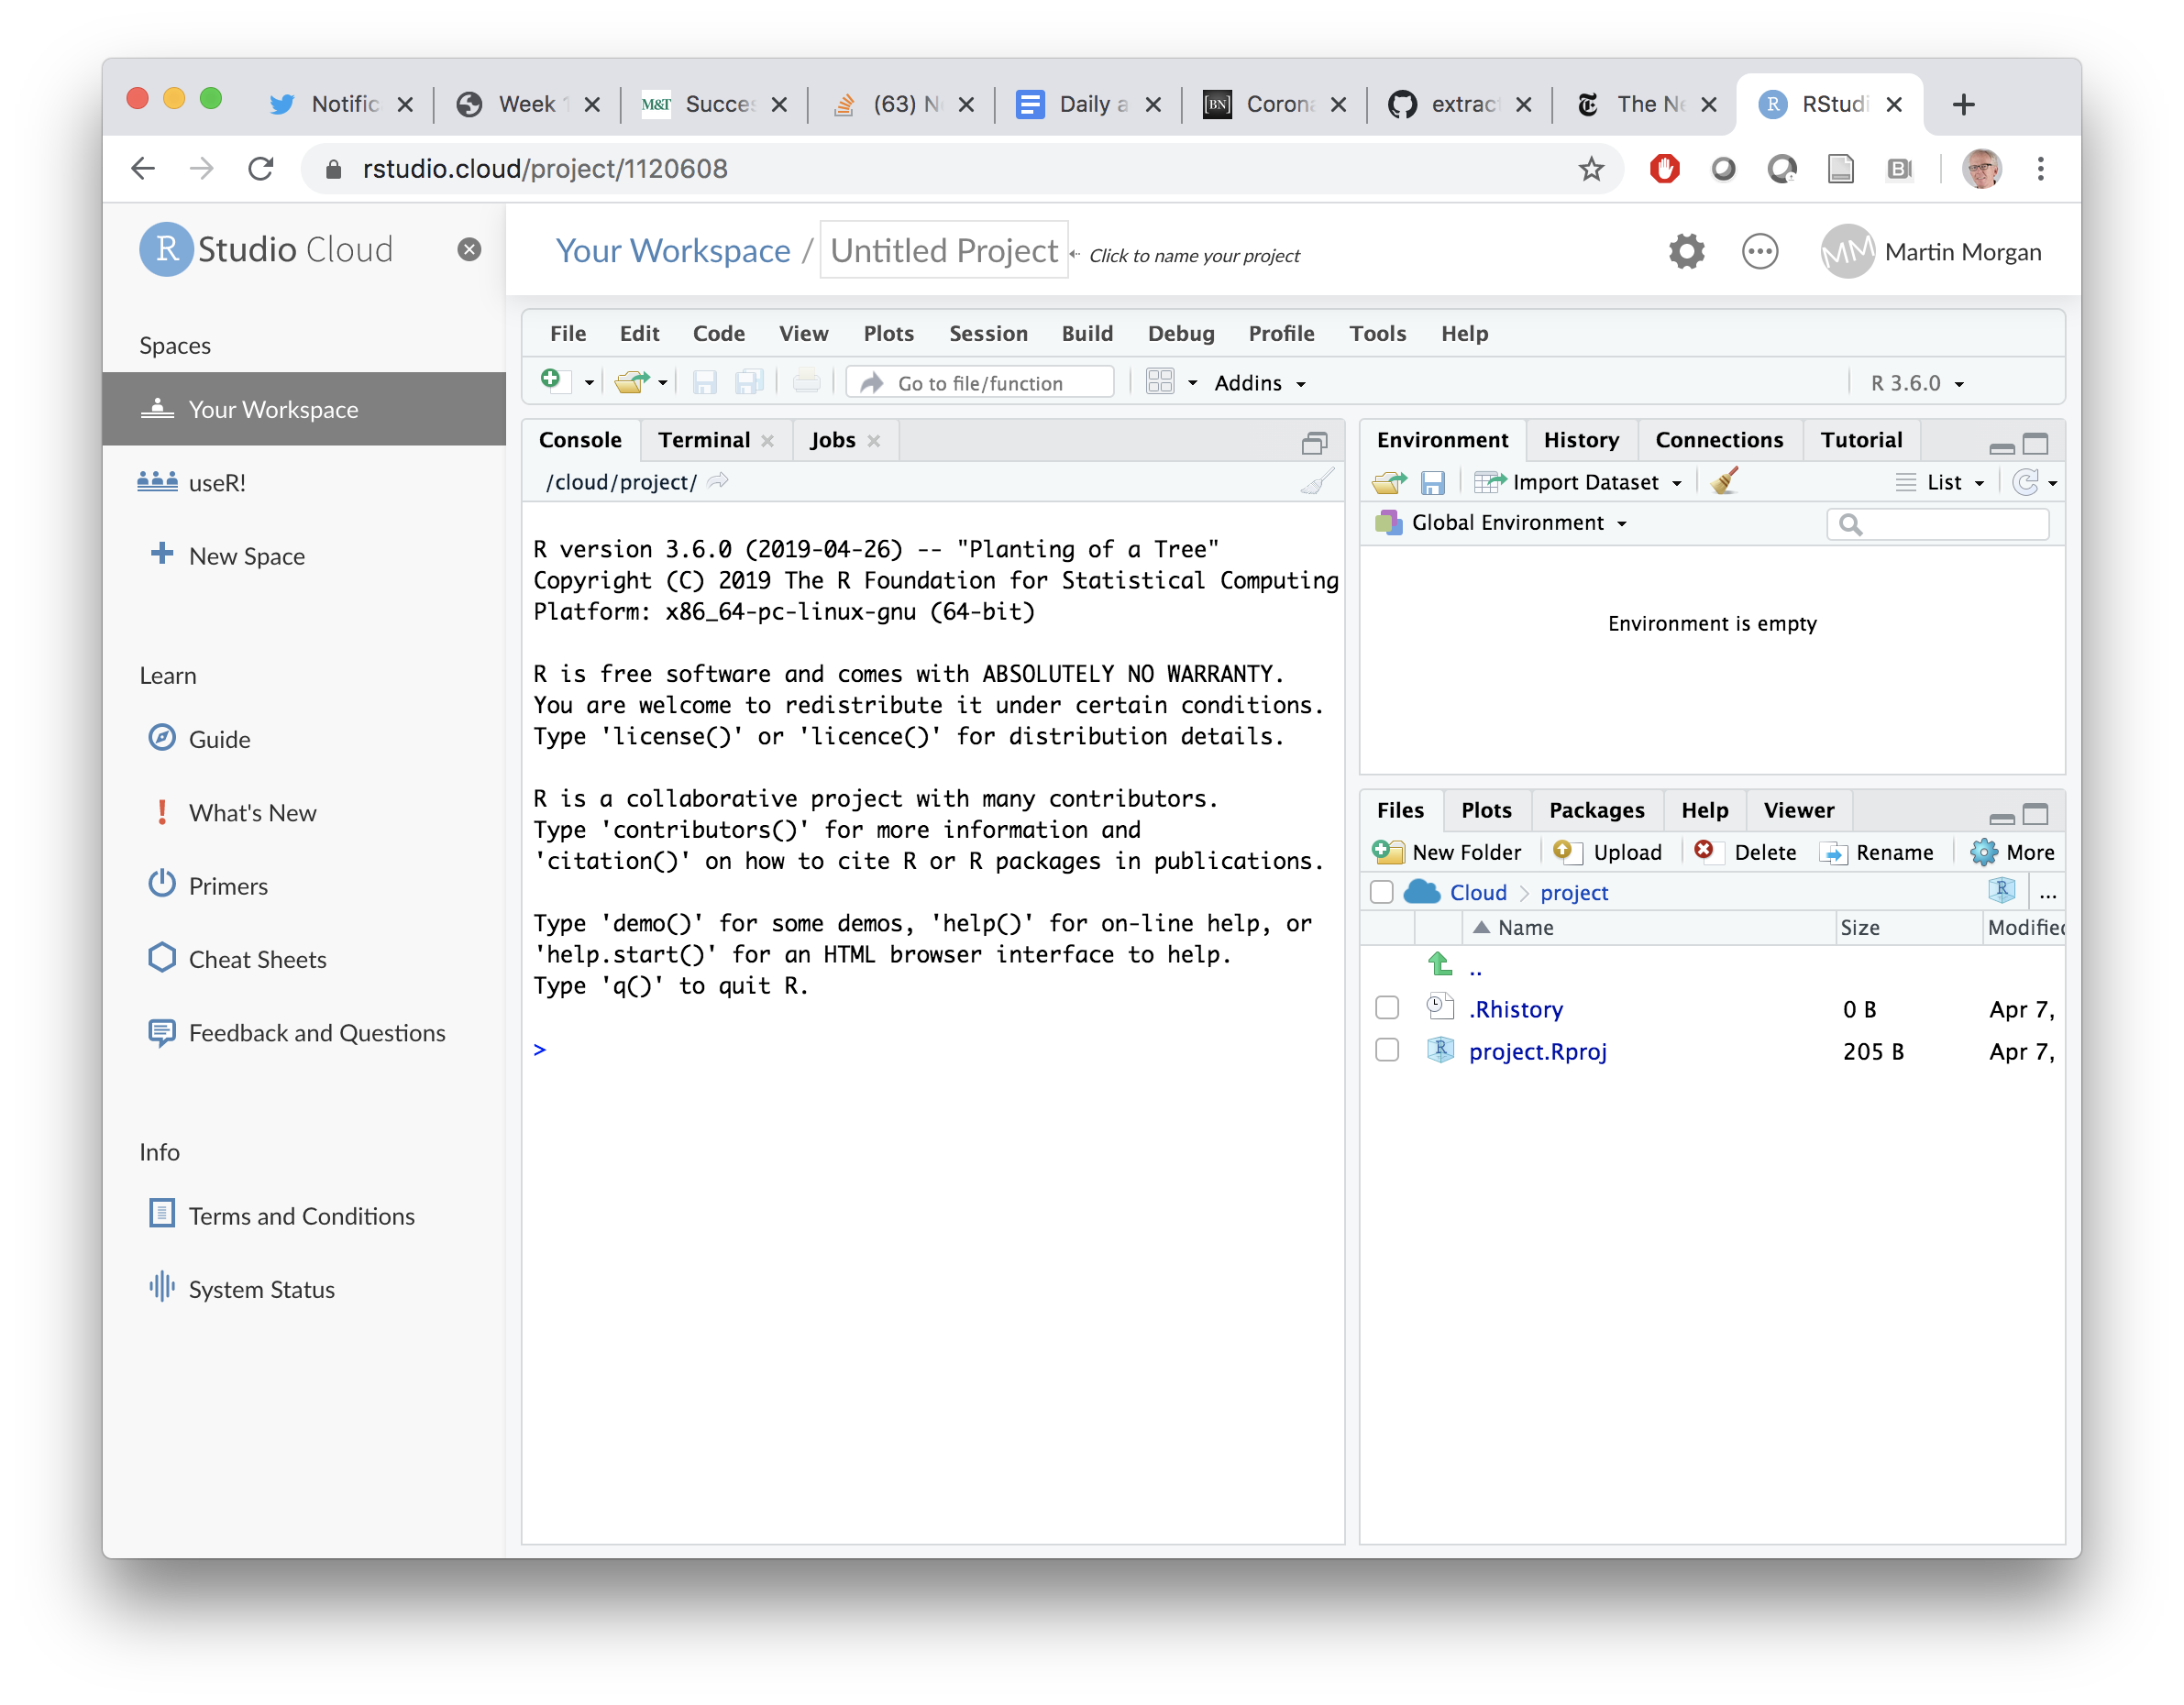
\includegraphics[width=33.08in]{images/RStudio-cloud-project}
\end{itemize}


\includegraphics[width=9.28in]{images/breakout_stop}

\hypertarget{breakout-room}{%
\subsubsection*{Breakout Room}\label{breakout-room}}
\addcontentsline{toc}{subsubsection}{Breakout Room}

At this point you should have RStudio running either via your desktop installation or through rstudio.cloud. If not, please let us know via the chat window and we'll invite you to a breakout room to troubleshoot your installation.

\hypertarget{basics-of-r-25-minutes}{%
\subsection{\texorpdfstring{Basics of \emph{R} (25 minutes)}{Basics of R (25 minutes)}}\label{basics-of-r-25-minutes}}

\hypertarget{r-as-a-simple-calculator}{%
\subsubsection*{R as a simple calculator}\label{r-as-a-simple-calculator}}
\addcontentsline{toc}{subsubsection}{R as a simple calculator}

\begin{Shaded}
\begin{Highlighting}[]
\DecValTok{1} \OperatorTok{+}\StringTok{ }\DecValTok{2}
\CommentTok{## [1] 3}
\end{Highlighting}
\end{Shaded}

\hypertarget{r-console-output}{%
\subsubsection*{R Console Output}\label{r-console-output}}
\addcontentsline{toc}{subsubsection}{R Console Output}

Enter this in the console:

\begin{Shaded}
\begin{Highlighting}[]
\DecValTok{2} \OperatorTok{+}\StringTok{ }\DecValTok{3} \OperatorTok{*}\StringTok{ }\DecValTok{5}
\CommentTok{## [1] 17}
\end{Highlighting}
\end{Shaded}

Q: what's the \texttt{{[}1{]}} all about in the output?

A: It's the index of the first entry in each line.

This is maybe a better example:

\begin{Shaded}
\begin{Highlighting}[]
\DecValTok{1}\OperatorTok{:}\DecValTok{30}
\CommentTok{##  [1]  1  2  3  4  5  6  7  8  9 10 11 12 13 14 15 16 17 18 19 20 21 22 23 24 25}
\CommentTok{## [26] 26 27 28 29 30}
\end{Highlighting}
\end{Shaded}

\hypertarget{displaying-help-in-the-r-console}{%
\subsubsection*{Displaying help in the R Console}\label{displaying-help-in-the-r-console}}
\addcontentsline{toc}{subsubsection}{Displaying help in the R Console}

\texttt{?\ \textless{}command-name\textgreater{}}

\begin{itemize}
\item
  Some examples:

\begin{verbatim}
? cat
? print
\end{verbatim}
\end{itemize}

\hypertarget{variables}{%
\subsubsection*{Variables}\label{variables}}
\addcontentsline{toc}{subsubsection}{Variables}

Naming variables in \emph{R}

\begin{itemize}
\item
  A variable name can contain letters, numbers, and the dot \texttt{.} or underline \texttt{\_} characters. Variables should start with a letter.
\item
  Try entering these in the console:

  \texttt{y\ =\ 2}

  \texttt{try.this\ =\ 33.3}

  \texttt{oneMoreTime\ =\ "woohoo"}
\item
  Now try these:

  \texttt{2y\ =\ 2}

  \texttt{\_z\ =\ 33.3}

  \texttt{function\ =\ "oops,\ my\ bad"}
\end{itemize}

\emph{R} is case sensitive (R != r)

\begin{Shaded}
\begin{Highlighting}[]
\NormalTok{R =}\StringTok{ }\DecValTok{2}
\NormalTok{r =}\StringTok{ }\DecValTok{3}
\NormalTok{R }\OperatorTok{==}\StringTok{ }\NormalTok{r}
\CommentTok{## [1] FALSE}
\end{Highlighting}
\end{Shaded}

Variable Assignment

\begin{itemize}
\item
  You may use \texttt{=} or \texttt{\textless{}-} (and even \texttt{-\textgreater{}}) to assign values to a variable.

\begin{Shaded}
\begin{Highlighting}[]
\NormalTok{x <-}\StringTok{ }\DecValTok{2} \OperatorTok{+}\StringTok{ }\DecValTok{3} \OperatorTok{*}\StringTok{ }\DecValTok{5}
\NormalTok{y =}\StringTok{  }\DecValTok{2} \OperatorTok{+}\StringTok{ }\DecValTok{3} \OperatorTok{*}\StringTok{ }\DecValTok{6}
\DecValTok{2} \OperatorTok{+}\StringTok{ }\DecValTok{3} \OperatorTok{*}\StringTok{ }\DecValTok{7}\NormalTok{ ->}\StringTok{ }\NormalTok{z}
\KeywordTok{cat}\NormalTok{(x, y, z)}
\CommentTok{## 17 20 23}
\end{Highlighting}
\end{Shaded}
\end{itemize}

\emph{R}'s four basic `atomic' data types

\begin{itemize}
\tightlist
\item
  Numeric (includes integer, double, etc.)

  \begin{itemize}
  \tightlist
  \item
    \texttt{3.14}, \texttt{1}, \texttt{2600}
  \end{itemize}
\item
  Character (string)

  \begin{itemize}
  \tightlist
  \item
    \texttt{"hey,\ I\textquotesingle{}m\ a\ string"}
  \item
    \texttt{\textquotesingle{}single\ quotes\ are\ ok\ too\textquotesingle{}}
  \end{itemize}
\item
  Logical

  \begin{itemize}
  \tightlist
  \item
    \texttt{TRUE} or \texttt{FALSE} (note all caps)
  \end{itemize}
\item
  \texttt{NA}

  \begin{itemize}
  \tightlist
  \item
    not assigned (no known value)
  \end{itemize}
\end{itemize}

Use \texttt{class()} to query the class of data:

\begin{Shaded}
\begin{Highlighting}[]
\NormalTok{a <-}\StringTok{ }\DecValTok{5}
\KeywordTok{class}\NormalTok{(a)}
\CommentTok{## [1] "numeric"}
\end{Highlighting}
\end{Shaded}

Use \texttt{as.} to coerce a variable to a specific data type

\begin{Shaded}
\begin{Highlighting}[]
\NormalTok{a <-}\StringTok{ }\KeywordTok{as.integer}\NormalTok{(}\DecValTok{5}\NormalTok{)}
\KeywordTok{class}\NormalTok{(a)}
\CommentTok{## [1] "integer"}
\end{Highlighting}
\end{Shaded}

\begin{Shaded}
\begin{Highlighting}[]
\NormalTok{d <-}\StringTok{ }\KeywordTok{as.logical}\NormalTok{(a)}
\NormalTok{d}
\CommentTok{## [1] TRUE}
\KeywordTok{class}\NormalTok{(d)}
\CommentTok{## [1] "logical"}
\end{Highlighting}
\end{Shaded}

\hypertarget{using-logical-operators}{%
\subsubsection*{Using Logical Operators}\label{using-logical-operators}}
\addcontentsline{toc}{subsubsection}{Using Logical Operators}

Equivalence test (\texttt{==}):

\begin{Shaded}
\begin{Highlighting}[]
\DecValTok{1} \OperatorTok{==}\StringTok{ }\DecValTok{2}
\CommentTok{## [1] FALSE}
\end{Highlighting}
\end{Shaded}

Not equal test (\texttt{!=}):

\begin{Shaded}
\begin{Highlighting}[]
\DecValTok{1} \OperatorTok{!=}\StringTok{ }\DecValTok{2}
\CommentTok{## [1] TRUE}
\end{Highlighting}
\end{Shaded}

less-than (\texttt{\textless{}}) and greater-than (\texttt{\textgreater{}}):

\begin{Shaded}
\begin{Highlighting}[]
\DecValTok{18} \OperatorTok{>}\StringTok{ }\DecValTok{44}
\CommentTok{## [1] FALSE}
\DecValTok{3} \OperatorTok{<}\StringTok{ }\DecValTok{204}
\CommentTok{## [1] TRUE}
\end{Highlighting}
\end{Shaded}

Logical Or (\texttt{\textbar{}}):

\begin{Shaded}
\begin{Highlighting}[]
\NormalTok{(}\DecValTok{1} \OperatorTok{==}\StringTok{ }\DecValTok{2}\NormalTok{) }\OperatorTok{|}\StringTok{ }\NormalTok{(}\DecValTok{2} \OperatorTok{==}\StringTok{ }\DecValTok{2}\NormalTok{)}
\CommentTok{## [1] TRUE}
\end{Highlighting}
\end{Shaded}

Logical And (\texttt{\&}):

\begin{Shaded}
\begin{Highlighting}[]
\NormalTok{(}\DecValTok{1} \OperatorTok{==}\StringTok{ }\DecValTok{2}\NormalTok{) }\OperatorTok{&}\StringTok{ }\NormalTok{(}\DecValTok{2} \OperatorTok{==}\StringTok{ }\DecValTok{2}\NormalTok{)}
\CommentTok{## [1] FALSE}
\end{Highlighting}
\end{Shaded}

\hypertarget{objects-and-vectors-in-r}{%
\subsubsection*{Objects and Vectors in R}\label{objects-and-vectors-in-r}}
\addcontentsline{toc}{subsubsection}{Objects and Vectors in R}

Objects

\begin{itemize}
\tightlist
\item
  R stores everything, variables included, in `objects'.
\end{itemize}

\begin{Shaded}
\begin{Highlighting}[]
\NormalTok{x <-}\StringTok{ }\FloatTok{2.71}

\CommentTok{# print the value of an object}
\KeywordTok{print}\NormalTok{(x)}
\CommentTok{## [1] 2.71}

\CommentTok{# determine class or internal type of an object}
\KeywordTok{class}\NormalTok{(x)}
\CommentTok{## [1] "numeric"}

\CommentTok{# TRUE if an object has not been assigned a value}
\KeywordTok{is.na}\NormalTok{(x)}
\CommentTok{## [1] FALSE}
\end{Highlighting}
\end{Shaded}

Vectors

\begin{itemize}
\tightlist
\item
  `Vectors' and `data frames' are the bread and butter of R
\item
  Vectors consist of several elements of the same class

  \begin{itemize}
  \tightlist
  \item
    e.g.~a vector of heart rates, one per patient
  \end{itemize}
\end{itemize}

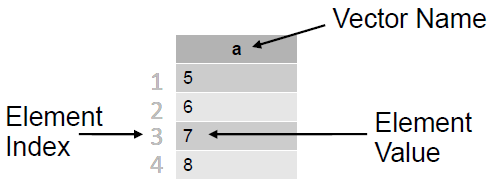
\includegraphics[width=6.85in]{images/simple_vector}

Data frames (\texttt{data.frame})

\begin{itemize}
\tightlist
\item
  Data frames are structures that can contain columns of various types

  \begin{itemize}
  \tightlist
  \item
    e.g.~height, weight, age, heart rate, etc.
  \item
    Handy containers for experimental data
  \item
    Analogous to spreadsheet data
  \item
    More on Data Frames throughout the week!
  \end{itemize}
\end{itemize}

\hypertarget{working-with-vectors}{%
\subsubsection*{Working with Vectors}\label{working-with-vectors}}
\addcontentsline{toc}{subsubsection}{Working with Vectors}

Creating a Vector

\begin{itemize}
\tightlist
\item
  Use the \texttt{c()} function
\end{itemize}

\begin{Shaded}
\begin{Highlighting}[]
\NormalTok{name <-}\StringTok{ }\KeywordTok{c}\NormalTok{(}\StringTok{"John Doe"}\NormalTok{, }\StringTok{"Jane Smith"}\NormalTok{, }\StringTok{"MacGillicuddy Jones"}\NormalTok{, }\StringTok{"Echo Shamus"}\NormalTok{)}
\NormalTok{age <-}\StringTok{ }\KeywordTok{c}\NormalTok{(}\DecValTok{36}\NormalTok{, }\DecValTok{54}\NormalTok{, }\DecValTok{82}\NormalTok{, }\DecValTok{15}\NormalTok{)}
\NormalTok{favorite_color <-}\StringTok{ }\KeywordTok{c}\NormalTok{(}\StringTok{"red"}\NormalTok{, }\StringTok{"orange"}\NormalTok{, }\StringTok{"green"}\NormalTok{, }\StringTok{"black"}\NormalTok{)}

\CommentTok{## print the vectors}
\NormalTok{name}
\CommentTok{## [1] "John Doe"            "Jane Smith"          "MacGillicuddy Jones"}
\CommentTok{## [4] "Echo Shamus"}
\NormalTok{age}
\CommentTok{## [1] 36 54 82 15}
\NormalTok{favorite_color}
\CommentTok{## [1] "red"    "orange" "green"  "black"}
\end{Highlighting}
\end{Shaded}

Accessing vector data

\begin{itemize}
\tightlist
\item
  Use numerical indexing
\item
  R uses 1-based indexing

  \begin{itemize}
  \tightlist
  \item
    1st vector element has index of 1
  \item
    2nd has an index of 2
  \item
    3rd has an index of 3
  \item
    and so on
  \end{itemize}
\end{itemize}

\begin{Shaded}
\begin{Highlighting}[]
\NormalTok{name[}\DecValTok{1}\NormalTok{]}
\CommentTok{## [1] "John Doe"}
\NormalTok{age[}\DecValTok{3}\NormalTok{]}
\CommentTok{## [1] 82}
\end{Highlighting}
\end{Shaded}

\begin{itemize}
\tightlist
\item
  R supports ``slicing'' (i.e.~extracting multiple items)
\end{itemize}

\begin{Shaded}
\begin{Highlighting}[]
\NormalTok{favorite_color[}\KeywordTok{c}\NormalTok{(}\DecValTok{2}\NormalTok{, }\DecValTok{3}\NormalTok{)]}
\CommentTok{## [1] "orange" "green"}
\end{Highlighting}
\end{Shaded}

\begin{itemize}
\tightlist
\item
  Negative indices are omitted
\end{itemize}

\begin{Shaded}
\begin{Highlighting}[]
\NormalTok{age[}\OperatorTok{-}\DecValTok{2}\NormalTok{]}
\CommentTok{## [1] 36 82 15}
\end{Highlighting}
\end{Shaded}

Some Useful Vector Operations

\begin{itemize}
\tightlist
\item
  \texttt{length()}: number of elements
\item
  \texttt{sum()}: sum of all element values
\item
  \texttt{unique()}: distinct values
\item
  \texttt{sort()}: sort elements, omitting NAs
\item
  \texttt{order()}: indices of sorted elements, NAs are last
\item
  \texttt{rev()}: reverse the order
\item
  \texttt{summary()}: simple statistics
\end{itemize}

\begin{Shaded}
\begin{Highlighting}[]
\NormalTok{a <-}\StringTok{ }\KeywordTok{c}\NormalTok{(}\DecValTok{5}\NormalTok{, }\DecValTok{5}\NormalTok{, }\DecValTok{6}\NormalTok{, }\DecValTok{7}\NormalTok{, }\DecValTok{8}\NormalTok{, }\DecValTok{4}\NormalTok{)}
\KeywordTok{sum}\NormalTok{(a)}
\CommentTok{## [1] 35}
\KeywordTok{length}\NormalTok{(a)}
\CommentTok{## [1] 6}
\KeywordTok{unique}\NormalTok{(a)}
\CommentTok{## [1] 5 6 7 8 4}
\KeywordTok{sort}\NormalTok{(a)}
\CommentTok{## [1] 4 5 5 6 7 8}
\KeywordTok{order}\NormalTok{(a)}
\CommentTok{## [1] 6 1 2 3 4 5}
\NormalTok{a[}\KeywordTok{order}\NormalTok{(a)]}
\CommentTok{## [1] 4 5 5 6 7 8}
\KeywordTok{rev}\NormalTok{(a)}
\CommentTok{## [1] 4 8 7 6 5 5}
\KeywordTok{summary}\NormalTok{(a)}
\CommentTok{##    Min. 1st Qu.  Median    Mean 3rd Qu.    Max. }
\CommentTok{##   4.000   5.000   5.500   5.833   6.750   8.000}
\end{Highlighting}
\end{Shaded}

Handling Missing Data

\begin{itemize}
\tightlist
\item
  First consider the reason(s) for the missing data

  \begin{itemize}
  \tightlist
  \item
    e.g.~concentrations that are below detectable levels?
  \end{itemize}
\item
  Sometimes NAs in data require special statistical methods
\item
  Other times we can safely discard / ignore NA entries
\item
  To remove NAs prior to a calculation:
\end{itemize}

\begin{Shaded}
\begin{Highlighting}[]
\NormalTok{y =}\StringTok{ }\KeywordTok{c}\NormalTok{(}\DecValTok{1}\NormalTok{,}\OtherTok{NA}\NormalTok{,}\DecValTok{3}\NormalTok{,}\DecValTok{2}\NormalTok{,}\OtherTok{NA}\NormalTok{)}
\KeywordTok{sum}\NormalTok{(y, }\DataTypeTok{na.rm=}\OtherTok{TRUE}\NormalTok{)}
\CommentTok{## [1] 6}
\end{Highlighting}
\end{Shaded}

\hypertarget{wrapping-up-day-1}{%
\subsubsection*{Wrapping up day 1}\label{wrapping-up-day-1}}
\addcontentsline{toc}{subsubsection}{Wrapping up day 1}

The goal for today was to rapidly cover some of the essential aspects of R programming. For the remainder of the week you'll work at your own pace to get more of a hands-on deep dive into this material. If you run into trouble please don't hesiate to ask for help via Teams (QuaRantine Team), slack (QuaRantine Course), or email (Drs. Matott and Morgan) --- whatever works best for you!

\hypertarget{day-2-vectors-and-variables}{%
\section{Day 2: Vectors and variables}\label{day-2-vectors-and-variables}}

Our overall goal for the next few days is to use \emph{R} to create a daily log of quarantine activities.

Our goal for today is to become familiar with \emph{R} vectors. Along the way we'll probably make data entry and other errors that will start to get us comfortable with \emph{R}.

If you run into problems, reach out to the slack channel for support!

The astronaut Scott Kelly said that to survive a year on the International Space Station he found it essential to

\begin{itemize}
\tightlist
\item
  Follow a schedule -- plan your day, and stick to the plan
\item
  Pace yourselves -- you've got a long time to accomplish tasks, so don't try to get everything done in the first week.
\item
  Go outside -- if Scott can head out to space, we should be able to make it to the back yard or around the block!
\item
  Get a hobby -- something not work related, and away from that evil little screen. Maybe it's as simple as rediscovering the joy of reading.
\item
  Keep a journal
\item
  Take time to connect -- on a human level, with people you work with and people you don't!
\item
  Listen to experts -- Scott talked about relying on the mission controllers; for us maybe that's watching webinars or taking courses in new topics!
\item
  Wash your hands!
\end{itemize}

I wanted to emphasize `follow a schedule' and `keep a journal'. How can \emph{R} help? Well, I want to create a short record of how I spend today, day 2 of my quarantine.

My first goal is to create \emph{vectors} describing things I plan to do today. Let's start with some of these. To get up to speed, type the following into the \emph{R} console, at the \texttt{\textgreater{}} prompt

\begin{Shaded}
\begin{Highlighting}[]
\DecValTok{1} \OperatorTok{+}\StringTok{ }\DecValTok{2}
\end{Highlighting}
\end{Shaded}

Press the carriage return and remind yourself that \emph{R} is a calculator, and knows how to work with numbers!

Now type an activity in your day, for instance I often start with

\begin{Shaded}
\begin{Highlighting}[]
\StringTok{"check e-mail"}
\end{Highlighting}
\end{Shaded}

Now try assigning that to a variable, and displaying the variable, e.g.,

\begin{Shaded}
\begin{Highlighting}[]
\NormalTok{activity <-}\StringTok{ "check e-mail"}
\NormalTok{activity}
\CommentTok{## [1] "check e-mail"}
\end{Highlighting}
\end{Shaded}

OK, likely you have several activities scheduled. Create a \emph{vector} of a few of
these by \texttt{c}oncatenating individual values

\begin{Shaded}
\begin{Highlighting}[]
\KeywordTok{c}\NormalTok{(}\StringTok{"check e-mail"}\NormalTok{, }\StringTok{"breakfast"}\NormalTok{, }\StringTok{"conference call"}\NormalTok{, }\StringTok{"webinar"}\NormalTok{, }\StringTok{"walk"}\NormalTok{)}
\CommentTok{## [1] "check e-mail"    "breakfast"       "conference call" "webinar"        }
\CommentTok{## [5] "walk"}
\end{Highlighting}
\end{Shaded}

Assign these to a variable

\begin{Shaded}
\begin{Highlighting}[]
\NormalTok{activity <-}\StringTok{ }\KeywordTok{c}\NormalTok{(}\StringTok{"check e-mail"}\NormalTok{, }\StringTok{"breakfast"}\NormalTok{, }\StringTok{"conference call"}\NormalTok{, }\StringTok{"webinar"}\NormalTok{, }\StringTok{"walk"}\NormalTok{)}
\NormalTok{activity}
\CommentTok{## [1] "check e-mail"    "breakfast"       "conference call" "webinar"        }
\CommentTok{## [5] "walk"}
\end{Highlighting}
\end{Shaded}

Create another vector, but this time the vector should contain the minutes spent on each activity

\begin{Shaded}
\begin{Highlighting}[]
\NormalTok{minutes <-}\StringTok{ }\KeywordTok{c}\NormalTok{(}\DecValTok{20}\NormalTok{, }\DecValTok{30}\NormalTok{, }\DecValTok{60}\NormalTok{, }\DecValTok{60}\NormalTok{, }\DecValTok{60}\NormalTok{)}
\NormalTok{minutes}
\CommentTok{## [1] 20 30 60 60 60}
\end{Highlighting}
\end{Shaded}

So I spent 20 minutes checking email, 30 minutes having breakfast and things like that, I was in a conference call for 60 minutes, and then attended a webinar where I learned new stuff for another 60 minutes. Finally I went for a walk to clear my head and remember why I'm doing things.

Apply some basic functions to the variables, e.g., use \texttt{length()} to demonstrate that you for each \texttt{activity} you have recorded the \texttt{minutes}.

\begin{Shaded}
\begin{Highlighting}[]
\KeywordTok{length}\NormalTok{(activity)}
\CommentTok{## [1] 5}
\KeywordTok{length}\NormalTok{(minutes)}
\CommentTok{## [1] 5}
\end{Highlighting}
\end{Shaded}

Use \texttt{tail()} to select the last two activities (or \texttt{head()} to select the first two\ldots{})

\begin{Shaded}
\begin{Highlighting}[]
\KeywordTok{tail}\NormalTok{(activity, }\DecValTok{2}\NormalTok{)}
\CommentTok{## [1] "webinar" "walk"}
\KeywordTok{tail}\NormalTok{(minutes, }\DecValTok{2}\NormalTok{)}
\CommentTok{## [1] 60 60}
\end{Highlighting}
\end{Shaded}

\emph{R} has other types of vectors. Create a logical vector that indicates whether each activity was `work' activity' or something you did for your own survival. We'll say that checking email is a work-related activity!

\begin{Shaded}
\begin{Highlighting}[]
\NormalTok{is_work <-}\StringTok{ }\KeywordTok{c}\NormalTok{(}\OtherTok{TRUE}\NormalTok{, }\OtherTok{FALSE}\NormalTok{, }\OtherTok{TRUE}\NormalTok{, }\OtherTok{TRUE}\NormalTok{, }\OtherTok{FALSE}\NormalTok{)}
\NormalTok{is_work}
\CommentTok{## [1]  TRUE FALSE  TRUE  TRUE FALSE}
\end{Highlighting}
\end{Shaded}

\hypertarget{day-3-factor-date-and-na}{%
\section{\texorpdfstring{Day 3: \texttt{factor()}, \texttt{Date()}, and \texttt{NA}}{Day 3: factor(), Date(), and NA}}\label{day-3-factor-date-and-na}}

Yesterday we learned about \texttt{character}, \texttt{numeric}, and \texttt{logical} vectors in \emph{R} (you may need to revisit previous notes and re-create these variables)

\begin{Shaded}
\begin{Highlighting}[]
\NormalTok{activity}
\CommentTok{## [1] "check e-mail"    "breakfast"       "conference call" "webinar"        }
\CommentTok{## [5] "walk"}
\NormalTok{minutes}
\CommentTok{## [1] 20 30 60 60 60}
\NormalTok{is_work}
\CommentTok{## [1]  TRUE FALSE  TRUE  TRUE FALSE}
\end{Highlighting}
\end{Shaded}

Today we will learn about slightly more complicated vectors.

We created the logical vector \texttt{is\_work} to classify each \texttt{activity} as either work-related or not. What if we had several different categories? For instance, we might want to classify the activities into categories inspired by astronaut Kelly's guidance. Categories might include: \texttt{connect} with others; go outside and \texttt{exercise}; \texttt{consult} experts; get a \texttt{hobby}; and (my own category, I guess) perform \texttt{essential} functions like eating and sleeping. So the values of \texttt{activity} could be classified as

\begin{Shaded}
\begin{Highlighting}[]
\NormalTok{classification <-}
\StringTok{    }\KeywordTok{c}\NormalTok{(}\StringTok{"connect"}\NormalTok{, }\StringTok{"essential"}\NormalTok{, }\StringTok{"connect"}\NormalTok{, }\StringTok{"consult"}\NormalTok{, }\StringTok{"exercise"}\NormalTok{)}
\end{Highlighting}
\end{Shaded}

I want to emphasize a difference between the \texttt{activity} and \texttt{classification} variables. I want \texttt{activity} to be a character vector that could contain any description of an activity. But I want \texttt{classification} to be terms only from a limited set of possibilities. In \emph{R}, I want \texttt{classification} to be a special type of vector called a \texttt{factor}, with the \emph{values} of the vector restricted to a set of possible \emph{levels} that I define. I create a factor by enumerating the possible \emph{levels} that the factor can take on

\begin{Shaded}
\begin{Highlighting}[]
\NormalTok{levels <-}\StringTok{ }\KeywordTok{c}\NormalTok{(}\StringTok{"connect"}\NormalTok{, }\StringTok{"exercise"}\NormalTok{, }\StringTok{"consult"}\NormalTok{, }\StringTok{"hobby"}\NormalTok{, }\StringTok{"essential"}\NormalTok{)}
\end{Highlighting}
\end{Shaded}

And then tell \emph{R} that the vector \texttt{classification} should be a factor with values taken from a particular set of levels

\begin{Shaded}
\begin{Highlighting}[]
\NormalTok{classification <-}\StringTok{ }\KeywordTok{factor}\NormalTok{(}
    \KeywordTok{c}\NormalTok{(}\StringTok{"connect"}\NormalTok{, }\StringTok{"essential"}\NormalTok{, }\StringTok{"connect"}\NormalTok{, }\StringTok{"consult"}\NormalTok{, }\StringTok{"exercise"}\NormalTok{),}
    \DataTypeTok{levels =}\NormalTok{ levels}
\NormalTok{)}
\NormalTok{classification}
\CommentTok{## [1] connect   essential connect   consult   exercise }
\CommentTok{## Levels: connect exercise consult hobby essential}
\end{Highlighting}
\end{Shaded}

Notice that activity (a character vector) displays differently from classification (a factor)

\begin{Shaded}
\begin{Highlighting}[]
\NormalTok{activity}
\CommentTok{## [1] "check e-mail"    "breakfast"       "conference call" "webinar"        }
\CommentTok{## [5] "walk"}
\NormalTok{classification}
\CommentTok{## [1] connect   essential connect   consult   exercise }
\CommentTok{## Levels: connect exercise consult hobby essential}
\end{Highlighting}
\end{Shaded}

Also, some of the levels (e.g., \texttt{hobby}) have not been part of our schedule yet, but the factor still `knows' about the level.

Notice also what happens when I try to use a value (\texttt{disconnect}) that is not a level of a factor

\begin{Shaded}
\begin{Highlighting}[]
\KeywordTok{factor}\NormalTok{(}\KeywordTok{c}\NormalTok{(}\StringTok{"connect"}\NormalTok{, }\StringTok{"disconnect"}\NormalTok{), }\DataTypeTok{levels =}\NormalTok{ levels)}
\CommentTok{## [1] connect <NA>   }
\CommentTok{## Levels: connect exercise consult hobby essential}
\end{Highlighting}
\end{Shaded}

The value with the unknown level is displayed as \texttt{NA}, for `not known'. \texttt{NA} values can be present in any vector, e.g.,

\begin{Shaded}
\begin{Highlighting}[]
\KeywordTok{c}\NormalTok{(}\DecValTok{1}\NormalTok{, }\DecValTok{2}\NormalTok{, }\OtherTok{NA}\NormalTok{, }\DecValTok{4}\NormalTok{)}
\CommentTok{## [1]  1  2 NA  4}
\KeywordTok{c}\NormalTok{(}\StringTok{"walk"}\NormalTok{, }\StringTok{"talk"}\NormalTok{, }\OtherTok{NA}\NormalTok{)}
\CommentTok{## [1] "walk" "talk" NA}
\KeywordTok{c}\NormalTok{(}\OtherTok{NA}\NormalTok{, }\OtherTok{TRUE}\NormalTok{, }\OtherTok{FALSE}\NormalTok{, }\OtherTok{TRUE}\NormalTok{, }\OtherTok{TRUE}\NormalTok{)}
\CommentTok{## [1]    NA  TRUE FALSE  TRUE  TRUE}
\end{Highlighting}
\end{Shaded}

This serves as an indication that the value is simply not available. Use \texttt{NA} rather than adopting some special code (e.g., `-99') to indicate when a value is not available.

One other type of vector we will work a lot with are dates. All of my activities are for today, so I'll start with a character vector with the same length as my activity vector, each indicating the date in a consistent month-day-year format

\begin{Shaded}
\begin{Highlighting}[]
\NormalTok{dates <-}\StringTok{ }\KeywordTok{c}\NormalTok{(}\StringTok{"04-14-2020"}\NormalTok{, }\StringTok{"04-14-2020"}\NormalTok{, }\StringTok{"04-14-2020"}\NormalTok{, }\StringTok{"04-14-2020"}\NormalTok{, }\StringTok{"04-14-2020"}\NormalTok{)}
\NormalTok{dates}
\CommentTok{## [1] "04-14-2020" "04-14-2020" "04-14-2020" "04-14-2020" "04-14-2020"}
\end{Highlighting}
\end{Shaded}

Incidentally, I could do this more efficiently using the \texttt{rep}licate function

\begin{Shaded}
\begin{Highlighting}[]
\KeywordTok{rep}\NormalTok{(}\StringTok{"04-14-2020"}\NormalTok{, }\DecValTok{5}\NormalTok{)}
\CommentTok{## [1] "04-14-2020" "04-14-2020" "04-14-2020" "04-14-2020" "04-14-2020"}
\end{Highlighting}
\end{Shaded}

And even better use \texttt{length()} to know for sure how many times I should replicate the character vector

\begin{Shaded}
\begin{Highlighting}[]
\KeywordTok{rep}\NormalTok{(}\StringTok{"04-14-2020"}\NormalTok{, }\KeywordTok{length}\NormalTok{(activity))}
\CommentTok{## [1] "04-14-2020" "04-14-2020" "04-14-2020" "04-14-2020" "04-14-2020"}
\end{Highlighting}
\end{Shaded}

\texttt{dates} is a character vector, but it has specially meaning as a calendar date, \emph{R} has a \texttt{Date} \emph{class} that knows how to work with dates, for instance to calculate the number of days between two dates. We will \emph{coerce} \texttt{date} to an object of class \texttt{Date} using a function \texttt{as.Date}. Here's our first attempt\ldots{}

\begin{Shaded}
\begin{Highlighting}[]
\KeywordTok{as.Date}\NormalTok{(dates)}
\end{Highlighting}
\end{Shaded}

\ldots{} but this results in an error:

\begin{verbatim}
Error in charToDate(x) :
  character string is not in a standard unambiguous format
\end{verbatim}

\emph{R} doesn't know the format (month-day-year) of the dates we provide. The solution is to add a second argument to \texttt{as.Date()}. The second argument is a character vector that describes the date format. The format we use is \texttt{"\%m-\%d-\%Y"}, which says that we provide the \texttt{\%m}onth first, then a hyphen, then the \texttt{\%d}ay, another hyphen, and finally the four-digit \texttt{\%Y}ear.

\begin{Shaded}
\begin{Highlighting}[]
\KeywordTok{as.Date}\NormalTok{(dates, }\DataTypeTok{format =} \StringTok{"%m-%d-%Y"}\NormalTok{)}
\CommentTok{## [1] "2020-04-14" "2020-04-14" "2020-04-14" "2020-04-14" "2020-04-14"}
\end{Highlighting}
\end{Shaded}

Notice that the format has been standardized to year-month-day. Also notice that although the original value of \texttt{date} and the return from \texttt{as.Data()} look the same, they are actually of different \emph{class}.

\begin{Shaded}
\begin{Highlighting}[]
\KeywordTok{class}\NormalTok{(date)}
\CommentTok{## [1] "function"}
\KeywordTok{class}\NormalTok{(}\KeywordTok{as.Date}\NormalTok{(dates, }\DataTypeTok{format =} \StringTok{"%m-%d-%Y"}\NormalTok{))}
\CommentTok{## [1] "Date"}
\end{Highlighting}
\end{Shaded}

\emph{R} will use the information about class to enable specialized calculation on dates, e.g., to sort them or to determine the number of days between different dates. So here's our \texttt{date} vector as a \texttt{Date} object.

\begin{Shaded}
\begin{Highlighting}[]
\NormalTok{dates <-}\StringTok{ }\KeywordTok{rep}\NormalTok{(}\StringTok{"04-14-2020"}\NormalTok{, }\KeywordTok{length}\NormalTok{(activity))}
\NormalTok{date <-}\StringTok{ }\KeywordTok{as.Date}\NormalTok{(dates, }\DataTypeTok{format =} \StringTok{"%m-%d-%Y"}\NormalTok{)}
\NormalTok{date}
\CommentTok{## [1] "2020-04-14" "2020-04-14" "2020-04-14" "2020-04-14" "2020-04-14"}
\end{Highlighting}
\end{Shaded}

OK, time for a walk! See you tomorrow!

\hypertarget{day-4-working-with-variables}{%
\section{Day 4: Working with variables}\label{day-4-working-with-variables}}

Remember that \emph{R} can act as a simple calculator, and that one can create new variables by assignment

\begin{Shaded}
\begin{Highlighting}[]
\NormalTok{x <-}\StringTok{ }\DecValTok{1}
\NormalTok{x }\OperatorTok{+}\StringTok{ }\DecValTok{1}
\CommentTok{## [1] 2}
\NormalTok{y <-}\StringTok{ }\NormalTok{x }\OperatorTok{+}\StringTok{ }\DecValTok{1}
\NormalTok{y}
\CommentTok{## [1] 2}
\end{Highlighting}
\end{Shaded}

Let's apply these ideaas to our \texttt{minutes} vector from earlier in the week.

\begin{Shaded}
\begin{Highlighting}[]
\NormalTok{minutes <-}\StringTok{ }\KeywordTok{c}\NormalTok{(}\DecValTok{20}\NormalTok{, }\DecValTok{30}\NormalTok{, }\DecValTok{60}\NormalTok{, }\DecValTok{60}\NormalTok{, }\DecValTok{60}\NormalTok{)}
\end{Highlighting}
\end{Shaded}

We can perform basic arithmetic on vectors. Suppose we wanted to increase the time of each activity by 5 minutes

\begin{Shaded}
\begin{Highlighting}[]
\NormalTok{minutes }\OperatorTok{+}\StringTok{ }\DecValTok{5}
\CommentTok{## [1] 25 35 65 65 65}
\end{Highlighting}
\end{Shaded}

or to increase the time of the first two activities by 5 minutes, and the last three activities by 10 minutes

\begin{Shaded}
\begin{Highlighting}[]
\NormalTok{minutes }\OperatorTok{+}\StringTok{ }\KeywordTok{c}\NormalTok{(}\DecValTok{5}\NormalTok{, }\DecValTok{5}\NormalTok{, }\DecValTok{10}\NormalTok{, }\DecValTok{10}\NormalTok{, }\DecValTok{10}\NormalTok{)}
\CommentTok{## [1] 25 35 70 70 70}
\end{Highlighting}
\end{Shaded}

\emph{R} has a very large number of \emph{functions} that can be used on vectors. For instance, the average time spent on activities is

\begin{Shaded}
\begin{Highlighting}[]
\KeywordTok{mean}\NormalTok{(minutes)}
\CommentTok{## [1] 46}
\end{Highlighting}
\end{Shaded}

while the total amount of time is

\begin{Shaded}
\begin{Highlighting}[]
\KeywordTok{sum}\NormalTok{(minutes)}
\CommentTok{## [1] 230}
\end{Highlighting}
\end{Shaded}

Explore other typical mathematical transformations, e.g., \texttt{log()}, \texttt{log10()}, \texttt{sqrt()} (square root), \ldots{} Check out the help pages for each, e.g., \texttt{?log}.

Explore the consequences of \texttt{NA} in a vector for functions like \texttt{mean()} and \texttt{sum()}.

\begin{Shaded}
\begin{Highlighting}[]
\NormalTok{x <-}\StringTok{ }\KeywordTok{c}\NormalTok{(}\DecValTok{1}\NormalTok{, }\DecValTok{2}\NormalTok{, }\OtherTok{NA}\NormalTok{, }\DecValTok{3}\NormalTok{)}
\KeywordTok{mean}\NormalTok{(x)}
\CommentTok{## [1] NA}
\end{Highlighting}
\end{Shaded}

\emph{R} is saying that, since there is an unknown (\texttt{NA}) value in the vector, it cannot possibly know what the mean is! Tell \emph{R} to remove the missing values before performing the calculation by adding the \texttt{na.rm\ =\ TRUE} argument

\begin{Shaded}
\begin{Highlighting}[]
\KeywordTok{mean}\NormalTok{(x, }\DataTypeTok{na.rm =} \OtherTok{TRUE}\NormalTok{)}
\CommentTok{## [1] 2}
\end{Highlighting}
\end{Shaded}

Check out the help page \texttt{?mean} to find a description of the \texttt{na.rm} and other arguments.

It's possible to perform logical operations on vectors, e.g., to ask which activities lasted 60 minutes or more

\begin{Shaded}
\begin{Highlighting}[]
\NormalTok{minutes }\OperatorTok{>=}\StringTok{ }\DecValTok{60}
\CommentTok{## [1] FALSE FALSE  TRUE  TRUE  TRUE}
\end{Highlighting}
\end{Shaded}

Here's our \texttt{activity} vector

\begin{Shaded}
\begin{Highlighting}[]
\NormalTok{activity <-}\StringTok{ }\KeywordTok{c}\NormalTok{(}\StringTok{"check e-mail"}\NormalTok{, }\StringTok{"breakfast"}\NormalTok{, }\StringTok{"conference call"}\NormalTok{, }\StringTok{"webinar"}\NormalTok{, }\StringTok{"walk"}\NormalTok{)}
\end{Highlighting}
\end{Shaded}

The elements of this vector are numbered from 1 to 5. We can create a new vector that is a subset of this vector using \texttt{{[}} and an integer index, e.g., the second activity is

\begin{Shaded}
\begin{Highlighting}[]
\NormalTok{activity[}\DecValTok{2}\NormalTok{]}
\CommentTok{## [1] "breakfast"}
\end{Highlighting}
\end{Shaded}

The index can actually be a vector, so we could choose the second and fourth activity as

\begin{Shaded}
\begin{Highlighting}[]
\NormalTok{index <-}\StringTok{ }\KeywordTok{c}\NormalTok{(}\DecValTok{2}\NormalTok{, }\DecValTok{4}\NormalTok{)}
\NormalTok{activity[index]}
\CommentTok{## [1] "breakfast" "webinar"}
\end{Highlighting}
\end{Shaded}

In fact, we can use logical vectors for subsetting. Consider the activities that take sixty minutes or longer:

\begin{Shaded}
\begin{Highlighting}[]
\NormalTok{index <-}\StringTok{ }\NormalTok{minutes }\OperatorTok{>=}\StringTok{ }\DecValTok{60}
\NormalTok{activity[index]}
\CommentTok{## [1] "conference call" "webinar"         "walk"}
\end{Highlighting}
\end{Shaded}

We had previously characterized the activities as `work' or otherwise.

\begin{Shaded}
\begin{Highlighting}[]
\NormalTok{is_work <-}\StringTok{ }\KeywordTok{c}\NormalTok{(}\OtherTok{TRUE}\NormalTok{, }\OtherTok{FALSE}\NormalTok{, }\OtherTok{TRUE}\NormalTok{, }\OtherTok{TRUE}\NormalTok{, }\OtherTok{FALSE}\NormalTok{)}
\end{Highlighting}
\end{Shaded}

Use \texttt{is\_work} to subset \texttt{activity} and identify the work-related activities

\begin{Shaded}
\begin{Highlighting}[]
\NormalTok{activity[is_work]}
\CommentTok{## [1] "check e-mail"    "conference call" "webinar"}
\end{Highlighting}
\end{Shaded}

How many minutes were work-related?

\begin{Shaded}
\begin{Highlighting}[]
\NormalTok{work_minutes <-}\StringTok{ }\NormalTok{minutes[is_work]}
\KeywordTok{sum}\NormalTok{(work_minutes)}
\CommentTok{## [1] 140}
\end{Highlighting}
\end{Shaded}

What about not work related? \texttt{!} negates logical vectors, so

\begin{Shaded}
\begin{Highlighting}[]
\NormalTok{is_work}
\CommentTok{## [1]  TRUE FALSE  TRUE  TRUE FALSE}
\OperatorTok{!}\NormalTok{is_work}
\CommentTok{## [1] FALSE  TRUE FALSE FALSE  TRUE}
\NormalTok{non_work_minutes <-}\StringTok{ }\NormalTok{minutes[}\OperatorTok{!}\NormalTok{is_work]}
\KeywordTok{sum}\NormalTok{(non_work_minutes)}
\CommentTok{## [1] 90}
\end{Highlighting}
\end{Shaded}

Note that it doesn't make sense to take the \texttt{mean()} of a character vector like \texttt{activity}, and \emph{R} signals a warning and returns \texttt{NA}

\begin{Shaded}
\begin{Highlighting}[]
\KeywordTok{mean}\NormalTok{(activity)}
\CommentTok{## Warning in mean.default(activity): argument is not numeric or logical: returning}
\CommentTok{## NA}
\CommentTok{## [1] NA}
\end{Highlighting}
\end{Shaded}

Nonetheless, there are many functions that \emph{do} work on character vectors, e.g., the number of letters in each element \texttt{nchar()}, or transformation to upper-case

\begin{Shaded}
\begin{Highlighting}[]
\KeywordTok{nchar}\NormalTok{(activity)}
\CommentTok{## [1] 12  9 15  7  4}
\KeywordTok{toupper}\NormalTok{(activity)}
\CommentTok{## [1] "CHECK E-MAIL"    "BREAKFAST"       "CONFERENCE CALL" "WEBINAR"        }
\CommentTok{## [5] "WALK"}
\end{Highlighting}
\end{Shaded}

\hypertarget{day-5-friday-zoom-check-in}{%
\section{Day 5 (Friday) Zoom check-in}\label{day-5-friday-zoom-check-in}}

\hypertarget{review-and-trouble-shoot-25-minutes-martin}{%
\subsection{Review and trouble shoot (25 minutes; Martin)}\label{review-and-trouble-shoot-25-minutes-martin}}

Data representations

\begin{itemize}
\item
  `Atomic' vectors

\begin{Shaded}
\begin{Highlighting}[]
\NormalTok{activity <-}\StringTok{ }\KeywordTok{c}\NormalTok{(}\StringTok{"check e-mail"}\NormalTok{, }\StringTok{"breakfast"}\NormalTok{, }\StringTok{"conference call"}\NormalTok{, }\StringTok{"webinar"}\NormalTok{, }\StringTok{"walk"}\NormalTok{)}
\NormalTok{minutes <-}\StringTok{ }\KeywordTok{c}\NormalTok{(}\DecValTok{20}\NormalTok{, }\DecValTok{30}\NormalTok{, }\DecValTok{60}\NormalTok{, }\DecValTok{60}\NormalTok{, }\DecValTok{60}\NormalTok{)}
\NormalTok{is_work <-}\StringTok{ }\KeywordTok{c}\NormalTok{(}\OtherTok{TRUE}\NormalTok{, }\OtherTok{FALSE}\NormalTok{, }\OtherTok{TRUE}\NormalTok{, }\OtherTok{TRUE}\NormalTok{, }\OtherTok{FALSE}\NormalTok{)}
\end{Highlighting}
\end{Shaded}
\item
  \texttt{factor()} and \texttt{date()}

\begin{Shaded}
\begin{Highlighting}[]
\NormalTok{levels <-}\StringTok{ }\KeywordTok{c}\NormalTok{(}\StringTok{"connect"}\NormalTok{, }\StringTok{"exercise"}\NormalTok{, }\StringTok{"consult"}\NormalTok{, }\StringTok{"hobby"}\NormalTok{, }\StringTok{"essential"}\NormalTok{)}
\NormalTok{classification <-}\StringTok{ }\KeywordTok{factor}\NormalTok{(}
    \KeywordTok{c}\NormalTok{(}\StringTok{"connect"}\NormalTok{, }\StringTok{"essential"}\NormalTok{, }\StringTok{"connect"}\NormalTok{, }\StringTok{"consult"}\NormalTok{, }\StringTok{"exercise"}\NormalTok{),}
    \DataTypeTok{levels =}\NormalTok{ levels}
\NormalTok{)}

\NormalTok{dates <-}\StringTok{ }\KeywordTok{rep}\NormalTok{(}\StringTok{"04-14-2020"}\NormalTok{, }\KeywordTok{length}\NormalTok{(activity))}
\NormalTok{date <-}\StringTok{ }\KeywordTok{as.Date}\NormalTok{(dates, }\DataTypeTok{format =} \StringTok{"%m-%d-%Y"}\NormalTok{)}
\end{Highlighting}
\end{Shaded}
\item
  missing values

\begin{Shaded}
\begin{Highlighting}[]
\NormalTok{x <-}\StringTok{ }\KeywordTok{c}\NormalTok{(}\DecValTok{1}\NormalTok{, }\DecValTok{3}\NormalTok{, }\OtherTok{NA}\NormalTok{, }\DecValTok{5}\NormalTok{)}
\KeywordTok{sum}\NormalTok{(x)}
\CommentTok{## [1] NA}
\KeywordTok{sum}\NormalTok{(x, }\DataTypeTok{na.rm =} \OtherTok{TRUE}\NormalTok{)}
\CommentTok{## [1] 9}

\KeywordTok{factor}\NormalTok{(}\KeywordTok{c}\NormalTok{(}\StringTok{"connect"}\NormalTok{, }\StringTok{"disconnect"}\NormalTok{), }\DataTypeTok{levels =}\NormalTok{ levels)}
\CommentTok{## [1] connect <NA>   }
\CommentTok{## Levels: connect exercise consult hobby essential}
\end{Highlighting}
\end{Shaded}
\item
  functions and logical operators

\begin{Shaded}
\begin{Highlighting}[]
\NormalTok{x <-}\StringTok{ }\KeywordTok{c}\NormalTok{(}\DecValTok{1}\NormalTok{, }\DecValTok{3}\NormalTok{, }\OtherTok{NA}\NormalTok{, }\DecValTok{5}\NormalTok{)}
\KeywordTok{sum}\NormalTok{(x)}
\CommentTok{## [1] NA}
\KeywordTok{sum}\NormalTok{(x, }\DataTypeTok{na.rm =} \OtherTok{TRUE}\NormalTok{)}
\CommentTok{## [1] 9}

\NormalTok{minutes }\OperatorTok{>=}\StringTok{ }\DecValTok{60}
\CommentTok{## [1] FALSE FALSE  TRUE  TRUE  TRUE}
\end{Highlighting}
\end{Shaded}
\end{itemize}

Subsetting vectors

\begin{itemize}
\item
  1-basaed numeric indexes

\begin{Shaded}
\begin{Highlighting}[]
\NormalTok{activity}
\CommentTok{## [1] "check e-mail"    "breakfast"       "conference call" "webinar"        }
\CommentTok{## [5] "walk"}

\NormalTok{idx <-}\StringTok{ }\KeywordTok{c}\NormalTok{(}\DecValTok{1}\NormalTok{, }\DecValTok{3}\NormalTok{, }\DecValTok{1}\NormalTok{)}
\NormalTok{activity[idx]}
\CommentTok{## [1] "check e-mail"    "conference call" "check e-mail"}
\end{Highlighting}
\end{Shaded}
\item
  logical index

\begin{Shaded}
\begin{Highlighting}[]
\NormalTok{is_work}
\CommentTok{## [1]  TRUE FALSE  TRUE  TRUE FALSE}
\NormalTok{activity[is_work]}
\CommentTok{## [1] "check e-mail"    "conference call" "webinar"}

\KeywordTok{sum}\NormalTok{(minutes[is_work])}
\CommentTok{## [1] 140}
\end{Highlighting}
\end{Shaded}
\item
  Maybe more interesting\ldots{}

\begin{Shaded}
\begin{Highlighting}[]
\NormalTok{short <-}\StringTok{ }\NormalTok{minutes }\OperatorTok{<}\StringTok{ }\DecValTok{60}
\NormalTok{short}
\CommentTok{## [1]  TRUE  TRUE FALSE FALSE FALSE}
\NormalTok{minutes[short]}
\CommentTok{## [1] 20 30}
\NormalTok{activity[short]}
\CommentTok{## [1] "check e-mail" "breakfast"}
\end{Highlighting}
\end{Shaded}
\end{itemize}

Other fun topics

\begin{itemize}
\item
  \texttt{\%in\%}: a \emph{binary operator} -- is each of the vector elements on the left-hand side \emph{in} the set of elements on the right hand side

\begin{Shaded}
\begin{Highlighting}[]
\NormalTok{fruits <-}\StringTok{ }\KeywordTok{c}\NormalTok{(}\StringTok{"banana"}\NormalTok{, }\StringTok{"apple"}\NormalTok{, }\StringTok{"grape"}\NormalTok{, }\StringTok{"orange"}\NormalTok{, }\StringTok{"kiwi"}\NormalTok{)}
\KeywordTok{c}\NormalTok{(}\StringTok{"apple"}\NormalTok{, }\StringTok{"orange"}\NormalTok{, }\StringTok{"hand sanitizer"}\NormalTok{) }\OperatorTok\StringTok{ }\NormalTok{fruits}
\CommentTok{## [1]  TRUE  TRUE FALSE}
\end{Highlighting}
\end{Shaded}
\item
  \emph{named} vectors (see \href{https://www2.census.gov/programs-surveys/popest/tables/2010-2019/state/totals/nst-est2019-01.xlsx}{Annual Estimates\ldots{}} table from \href{https://www.census.gov/data/datasets/time-series/demo/popest/2010s-state-total.html}{census.gov})

  Define a named vector

\begin{Shaded}
\begin{Highlighting}[]
\NormalTok{state_populations <-}\StringTok{ }\KeywordTok{c}\NormalTok{(}
    \DataTypeTok{Alabama =} \DecValTok{4903185}\NormalTok{, }\DataTypeTok{Alaska =} \DecValTok{731545}\NormalTok{, }\DataTypeTok{Arizona =} \DecValTok{7278717}\NormalTok{, }\DataTypeTok{Arkansas =} \DecValTok{3017804}\NormalTok{,}
    \DataTypeTok{California =} \DecValTok{39512223}\NormalTok{, }\DataTypeTok{Colorado =} \DecValTok{5758736}\NormalTok{, }\DataTypeTok{Connecticut =} \DecValTok{3565287}\NormalTok{,}
    \DataTypeTok{Delaware =} \DecValTok{973764}\NormalTok{, }\StringTok{`}\DataTypeTok{District of Columbia}\StringTok{`}\NormalTok{ =}\StringTok{ }\DecValTok{705749}\NormalTok{, }\DataTypeTok{Florida =} \DecValTok{21477737}\NormalTok{,}
    \DataTypeTok{Georgia =} \DecValTok{10617423}\NormalTok{, }\DataTypeTok{Hawaii =} \DecValTok{1415872}\NormalTok{, }\DataTypeTok{Idaho =} \DecValTok{1787065}\NormalTok{, }\DataTypeTok{Illinois =} \DecValTok{12671821}\NormalTok{,}
    \DataTypeTok{Indiana =} \DecValTok{6732219}\NormalTok{, }\DataTypeTok{Iowa =} \DecValTok{3155070}\NormalTok{, }\DataTypeTok{Kansas =} \DecValTok{2913314}\NormalTok{, }\DataTypeTok{Kentucky =} \DecValTok{4467673}\NormalTok{,}
    \DataTypeTok{Louisiana =} \DecValTok{4648794}\NormalTok{, }\DataTypeTok{Maine =} \DecValTok{1344212}\NormalTok{, }\DataTypeTok{Maryland =} \DecValTok{6045680}\NormalTok{, }\DataTypeTok{Massachusetts =} \DecValTok{6892503}\NormalTok{,}
    \DataTypeTok{Michigan =} \DecValTok{9986857}\NormalTok{, }\DataTypeTok{Minnesota =} \DecValTok{5639632}\NormalTok{, }\DataTypeTok{Mississippi =} \DecValTok{2976149}\NormalTok{,}
    \DataTypeTok{Missouri =} \DecValTok{6137428}\NormalTok{, }\DataTypeTok{Montana =} \DecValTok{1068778}\NormalTok{, }\DataTypeTok{Nebraska =} \DecValTok{1934408}\NormalTok{, }\DataTypeTok{Nevada =} \DecValTok{3080156}\NormalTok{,}
    \StringTok{`}\DataTypeTok{New Hampshire}\StringTok{`}\NormalTok{ =}\StringTok{ }\DecValTok{1359711}\NormalTok{, }\StringTok{`}\DataTypeTok{New Jersey}\StringTok{`}\NormalTok{ =}\StringTok{ }\DecValTok{8882190}\NormalTok{, }\StringTok{`}\DataTypeTok{New Mexico}\StringTok{`}\NormalTok{ =}\StringTok{ }\DecValTok{2096829}\NormalTok{,}
    \StringTok{`}\DataTypeTok{New York}\StringTok{`}\NormalTok{ =}\StringTok{ }\DecValTok{19453561}\NormalTok{, }\StringTok{`}\DataTypeTok{North Carolina}\StringTok{`}\NormalTok{ =}\StringTok{ }\DecValTok{10488084}\NormalTok{, }\StringTok{`}\DataTypeTok{North Dakota}\StringTok{`}\NormalTok{ =}\StringTok{ }\DecValTok{762062}\NormalTok{,}
    \DataTypeTok{Ohio =} \DecValTok{11689100}\NormalTok{, }\DataTypeTok{Oklahoma =} \DecValTok{3956971}\NormalTok{, }\DataTypeTok{Oregon =} \DecValTok{4217737}\NormalTok{, }\DataTypeTok{Pennsylvania =} \DecValTok{12801989}\NormalTok{,}
    \StringTok{`}\DataTypeTok{Rhode Island}\StringTok{`}\NormalTok{ =}\StringTok{ }\DecValTok{1059361}\NormalTok{, }\StringTok{`}\DataTypeTok{South Carolina}\StringTok{`}\NormalTok{ =}\StringTok{ }\DecValTok{5148714}\NormalTok{, }\StringTok{`}\DataTypeTok{South Dakota}\StringTok{`}\NormalTok{ =}\StringTok{ }\DecValTok{884659}\NormalTok{,}
    \DataTypeTok{Tennessee =} \DecValTok{6829174}\NormalTok{, }\DataTypeTok{Texas =} \DecValTok{28995881}\NormalTok{, }\DataTypeTok{Utah =} \DecValTok{3205958}\NormalTok{, }\DataTypeTok{Vermont =} \DecValTok{623989}\NormalTok{,}
    \DataTypeTok{Virginia =} \DecValTok{8535519}\NormalTok{, }\DataTypeTok{Washington =} \DecValTok{7614893}\NormalTok{, }\StringTok{`}\DataTypeTok{West Virginia}\StringTok{`}\NormalTok{ =}\StringTok{ }\DecValTok{1792147}\NormalTok{,}
    \DataTypeTok{Wisconsin =} \DecValTok{5822434}\NormalTok{, }\DataTypeTok{Wyoming =} \DecValTok{578759}
\NormalTok{)}
\end{Highlighting}
\end{Shaded}

  Computations

\begin{Shaded}
\begin{Highlighting}[]
\CommentTok{## US population}
\KeywordTok{sum}\NormalTok{(state_populations)}
\CommentTok{## [1] 328239523}

\CommentTok{## smallest states}
\KeywordTok{head}\NormalTok{(}\KeywordTok{sort}\NormalTok{(state_populations))}
\CommentTok{##              Wyoming              Vermont District of Columbia }
\CommentTok{##               578759               623989               705749 }
\CommentTok{##               Alaska         North Dakota         South Dakota }
\CommentTok{##               731545               762062               884659}

\CommentTok{## largest states}
\KeywordTok{head}\NormalTok{(}\KeywordTok{sort}\NormalTok{(state_populations, }\DataTypeTok{decreasing =} \OtherTok{TRUE}\NormalTok{))}
\CommentTok{##   California        Texas      Florida     New York Pennsylvania     Illinois }
\CommentTok{##     39512223     28995881     21477737     19453561     12801989     12671821}

\CommentTok{## states with more than 10 million people}
\NormalTok{big <-}\StringTok{ }\NormalTok{state_populations[state_populations }\OperatorTok{>}\StringTok{ }\DecValTok{10000000}\NormalTok{]}
\NormalTok{big}
\CommentTok{##     California        Florida        Georgia       Illinois       New York }
\CommentTok{##       39512223       21477737       10617423       12671821       19453561 }
\CommentTok{## North Carolina           Ohio   Pennsylvania          Texas }
\CommentTok{##       10488084       11689100       12801989       28995881}
\KeywordTok{names}\NormalTok{(big)}
\CommentTok{## [1] "California"     "Florida"        "Georgia"        "Illinois"      }
\CommentTok{## [5] "New York"       "North Carolina" "Ohio"           "Pennsylvania"  }
\CommentTok{## [9] "Texas"}
\end{Highlighting}
\end{Shaded}

  Subset by name

\begin{Shaded}
\begin{Highlighting}[]
\CommentTok{## populations of California and New York}
\NormalTok{state_populations[}\KeywordTok{c}\NormalTok{(}\StringTok{"California"}\NormalTok{, }\StringTok{"New York"}\NormalTok{)]}
\CommentTok{## California   New York }
\CommentTok{##   39512223   19453561}
\end{Highlighting}
\end{Shaded}
\end{itemize}

\hypertarget{weekend-activities-25-minutes-shawn}{%
\subsection{Weekend activities (25 minutes; Shawn)}\label{weekend-activities-25-minutes-shawn}}

Writing \emph{R} scripts

Saving data

\hypertarget{r-scripts}{%
\subsubsection*{R Scripts}\label{r-scripts}}
\addcontentsline{toc}{subsubsection}{R Scripts}

\hypertarget{day-6-r-scripts}{%
\section{\texorpdfstring{Day 6: \emph{R} scripts}{Day 6: R scripts}}\label{day-6-r-scripts}}

Some of you may have already started saving your R commands as script files. As the material gets more complicated (and more interesting) everyone will want to start doing this. Here is an example to get you started:

\begin{itemize}
\tightlist
\item
  In RStudio, click ``File --\textgreater{} New File --\textgreater{} R Script'' to create a new script file and open it in the editor
\end{itemize}

\begin{center}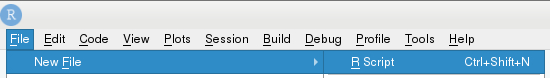
\includegraphics[width=0.6\linewidth]{images/rstudio_new_rscript_file} \end{center}

\begin{itemize}
\tightlist
\item
  By convention, R scripts have a .R exstension (e.g.~my\_script.R)

  \begin{itemize}
  \tightlist
  \item
    In RStudio, click into your untitled script and click ``File --\textgreater{} Save''
  \item
    Name your file something fun like \texttt{my\_first\_script.R} and save it
  \end{itemize}
\item
  Use the \texttt{\#} character for comments. Enter the following into your R Script file:
\end{itemize}

\begin{Shaded}
\begin{Highlighting}[]
\CommentTok{## This is my first R script}
\end{Highlighting}
\end{Shaded}

\begin{itemize}
\tightlist
\item
  Enter each command on a separate line. It's also possible to enter multiple (short!) commands on a single line, separated by a semi-colon \texttt{;}
\end{itemize}

\begin{Shaded}
\begin{Highlighting}[]
\NormalTok{x =}\StringTok{ "Hello world!"}
\NormalTok{y =}\StringTok{ 'Today is'}\NormalTok{; d =}\StringTok{ }\KeywordTok{format}\NormalTok{(}\KeywordTok{Sys.Date}\NormalTok{(), }\StringTok{"%b %d, %Y"}\NormalTok{)}
\KeywordTok{cat}\NormalTok{(x, y, d)}
\end{Highlighting}
\end{Shaded}

\begin{itemize}
\tightlist
\item
  Use the ``Run'' button in RStudio to run the highlighted portion of an R script file. Try this on your simple R Script.
\end{itemize}

\begin{center}
\includegraphics[width=0.8\linewidth]{images/rstudio_run_button} \end{center}

\begin{Shaded}
\begin{Highlighting}[]
\NormalTok{x =}\StringTok{ "Hello world!"}\NormalTok{; y =}\StringTok{ 'Today is'}\NormalTok{; d =}\StringTok{ }\KeywordTok{format}\NormalTok{(}\KeywordTok{Sys.Date}\NormalTok{(),}\StringTok{"%b %d, %Y"}\NormalTok{)}
\KeywordTok{cat}\NormalTok{(x, y, d, }\StringTok{"}\CharTok{\textbackslash{}n}\StringTok{"}\NormalTok{)}
\CommentTok{## Hello world! Today is Apr 15, 2020}
\end{Highlighting}
\end{Shaded}

\begin{itemize}
\tightlist
\item
  Alternatively, use ``Run --\textgreater{} Run All'' to run an entire script file.
\end{itemize}

For today's exercise, create a script file that summarizes your quarantine activities over several days. Use comments, white space (blank lines and spaces), and variable names to summarize each day. Here's what I've got\ldots{}

\begin{Shaded}
\begin{Highlighting}[]
\CommentTok{## 'classification' factor levels}
\NormalTok{levels <-}\StringTok{ }\KeywordTok{c}\NormalTok{(}\StringTok{"connect"}\NormalTok{, }\StringTok{"exercise"}\NormalTok{, }\StringTok{"consult"}\NormalTok{, }\StringTok{"hobby"}\NormalTok{, }\StringTok{"essential"}\NormalTok{)}

\CommentTok{## Quarantine log, day 1}

\NormalTok{activity_day_}\DecValTok{1}\NormalTok{ <-}
\StringTok{    }\KeywordTok{c}\NormalTok{(}\StringTok{"check e-mail"}\NormalTok{, }\StringTok{"breakfast"}\NormalTok{, }\StringTok{"conference call"}\NormalTok{, }\StringTok{"webinar"}\NormalTok{, }\StringTok{"walk"}\NormalTok{)}
\NormalTok{minutes_day_}\DecValTok{2}\NormalTok{ <-}\StringTok{ }\KeywordTok{c}\NormalTok{(}\DecValTok{20}\NormalTok{, }\DecValTok{30}\NormalTok{, }\DecValTok{60}\NormalTok{, }\DecValTok{60}\NormalTok{, }\DecValTok{60}\NormalTok{)}
\NormalTok{is_work_day_}\DecValTok{2}\NormalTok{ <-}\StringTok{ }\KeywordTok{c}\NormalTok{(}\OtherTok{TRUE}\NormalTok{, }\OtherTok{FALSE}\NormalTok{, }\OtherTok{TRUE}\NormalTok{, }\OtherTok{TRUE}\NormalTok{, }\OtherTok{FALSE}\NormalTok{)}
\NormalTok{classification_day_}\DecValTok{2}\NormalTok{ <-}\StringTok{ }\KeywordTok{factor}\NormalTok{(}
    \KeywordTok{c}\NormalTok{(}\StringTok{"connect"}\NormalTok{, }\StringTok{"essential"}\NormalTok{, }\StringTok{"connect"}\NormalTok{, }\StringTok{"consult"}\NormalTok{, }\StringTok{"exercise"}\NormalTok{),}
    \DataTypeTok{levels =}\NormalTok{ levels}
\NormalTok{)}
\NormalTok{date_day_}\DecValTok{1}\NormalTok{ <-}\StringTok{ }\KeywordTok{as.Date}\NormalTok{(}\KeywordTok{rep}\NormalTok{(}\StringTok{"04-14-2020"}\NormalTok{, }\KeywordTok{length}\NormalTok{(activity_day_}\DecValTok{1}\NormalTok{)), }\StringTok{"%m-%d-%Y"}\NormalTok{)}

\CommentTok{## Quarantine log, day 2}

\NormalTok{activity_day_}\DecValTok{2}\NormalTok{ <-}
\StringTok{    }\KeywordTok{c}\NormalTok{(}\StringTok{"check e-mail"}\NormalTok{, }\StringTok{"breakfast"}\NormalTok{, }\StringTok{"conference call"}\NormalTok{, }\StringTok{"webinar"}\NormalTok{, }\StringTok{"read a book"}\NormalTok{)}
\NormalTok{minutes_day_}\DecValTok{2}\NormalTok{ <-}\StringTok{ }\KeywordTok{c}\NormalTok{(}\DecValTok{20}\NormalTok{, }\DecValTok{30}\NormalTok{, }\DecValTok{60}\NormalTok{, }\DecValTok{60}\NormalTok{, }\DecValTok{60}\NormalTok{)}
\NormalTok{is_work_day_}\DecValTok{2}\NormalTok{ <-}\StringTok{ }\KeywordTok{c}\NormalTok{(}\OtherTok{TRUE}\NormalTok{, }\OtherTok{FALSE}\NormalTok{, }\OtherTok{TRUE}\NormalTok{, }\OtherTok{TRUE}\NormalTok{, }\OtherTok{FALSE}\NormalTok{)}
\NormalTok{classification_day_}\DecValTok{2}\NormalTok{ <-}\StringTok{ }\KeywordTok{factor}\NormalTok{(}
    \KeywordTok{c}\NormalTok{(}\StringTok{"connect"}\NormalTok{, }\StringTok{"essential"}\NormalTok{, }\StringTok{"connect"}\NormalTok{, }\StringTok{"consult"}\NormalTok{, }\StringTok{"hobby"}\NormalTok{),}
    \DataTypeTok{levels =}\NormalTok{ levels}
\NormalTok{)}
\NormalTok{date_day_}\DecValTok{2}\NormalTok{ <-}\StringTok{ }\KeywordTok{as.Date}\NormalTok{(}\KeywordTok{rep}\NormalTok{(}\StringTok{"04-15-2020"}\NormalTok{, }\KeywordTok{length}\NormalTok{(activity_day_}\DecValTok{2}\NormalTok{)), }\StringTok{"%m-%d-%Y"}\NormalTok{)}

\CommentTok{## Quarantine log, day 3}

\NormalTok{activity_day_}\DecValTok{3}\NormalTok{ <-}
\StringTok{    }\KeywordTok{c}\NormalTok{(}\StringTok{"check e-mail"}\NormalTok{, }\StringTok{"breakfast"}\NormalTok{, }\StringTok{"webinar"}\NormalTok{, }\StringTok{"read a book"}\NormalTok{)}
\NormalTok{minutes_day_}\DecValTok{3}\NormalTok{ <-}\StringTok{ }\KeywordTok{c}\NormalTok{(}\DecValTok{20}\NormalTok{, }\DecValTok{30}\NormalTok{, }\DecValTok{60}\NormalTok{, }\DecValTok{60}\NormalTok{)}
\NormalTok{is_work_day_}\DecValTok{3}\NormalTok{ <-}\StringTok{ }\KeywordTok{c}\NormalTok{(}\OtherTok{TRUE}\NormalTok{, }\OtherTok{FALSE}\NormalTok{, }\OtherTok{TRUE}\NormalTok{, }\OtherTok{FALSE}\NormalTok{)}
\NormalTok{classification_day_}\DecValTok{3}\NormalTok{ <-}\StringTok{ }\KeywordTok{factor}\NormalTok{(}
    \KeywordTok{c}\NormalTok{(}\StringTok{"connect"}\NormalTok{, }\StringTok{"essential"}\NormalTok{, }\StringTok{"connect"}\NormalTok{, }\StringTok{"consult"}\NormalTok{, }\StringTok{"hobby"}\NormalTok{),}
    \DataTypeTok{levels =}\NormalTok{ levels}
\NormalTok{)}
\NormalTok{date_day_}\DecValTok{3}\NormalTok{ <-}\StringTok{ }\KeywordTok{as.Date}\NormalTok{(}\KeywordTok{rep}\NormalTok{(}\StringTok{"04-16-2020"}\NormalTok{, }\KeywordTok{length}\NormalTok{(activity_day_}\DecValTok{3}\NormalTok{)), }\StringTok{"%m-%d-%Y"}\NormalTok{)}
\end{Highlighting}
\end{Shaded}

Try \texttt{c}oncatenating these values, e.g.,

\begin{Shaded}
\begin{Highlighting}[]
\NormalTok{activity <-}\StringTok{ }\KeywordTok{c}\NormalTok{(activity_day_}\DecValTok{1}\NormalTok{, activity_day_}\DecValTok{2}\NormalTok{, activity_day_}\DecValTok{3}\NormalTok{)}
\NormalTok{activity}
\CommentTok{##  [1] "check e-mail"    "breakfast"       "conference call" "webinar"        }
\CommentTok{##  [5] "walk"            "check e-mail"    "breakfast"       "conference call"}
\CommentTok{##  [9] "webinar"         "read a book"     "check e-mail"    "breakfast"      }
\CommentTok{## [13] "webinar"         "read a book"}
\end{Highlighting}
\end{Shaded}

Save your script, quit \emph{R} and \emph{RStudio}, and restart \emph{R}. Re-open and run the script to re-do your original work.

Think about how this makes your work \emph{reproducible} from one day to the next, and how making your scientific work reproducible would be advantageous.

\hypertarget{day-7-saving-data}{%
\section{Day 7: Saving data}\label{day-7-saving-data}}

We've defined these variables

\begin{Shaded}
\begin{Highlighting}[]
\NormalTok{activity <-}\StringTok{ }\KeywordTok{c}\NormalTok{(}\StringTok{"check e-mail"}\NormalTok{, }\StringTok{"breakfast"}\NormalTok{, }\StringTok{"conference call"}\NormalTok{, }\StringTok{"webinar"}\NormalTok{, }\StringTok{"walk"}\NormalTok{)}
\NormalTok{minutes <-}\StringTok{ }\KeywordTok{c}\NormalTok{(}\DecValTok{20}\NormalTok{, }\DecValTok{30}\NormalTok{, }\DecValTok{60}\NormalTok{, }\DecValTok{60}\NormalTok{, }\DecValTok{60}\NormalTok{)}
\NormalTok{is_work <-}\StringTok{ }\KeywordTok{c}\NormalTok{(}\OtherTok{TRUE}\NormalTok{, }\OtherTok{FALSE}\NormalTok{, }\OtherTok{TRUE}\NormalTok{, }\OtherTok{TRUE}\NormalTok{, }\OtherTok{FALSE}\NormalTok{)}

\NormalTok{levels <-}\StringTok{ }\KeywordTok{c}\NormalTok{(}\StringTok{"connect"}\NormalTok{, }\StringTok{"exercise"}\NormalTok{, }\StringTok{"consult"}\NormalTok{, }\StringTok{"hobby"}\NormalTok{, }\StringTok{"essential"}\NormalTok{)}
\NormalTok{classification <-}\StringTok{ }\KeywordTok{factor}\NormalTok{(}
    \KeywordTok{c}\NormalTok{(}\StringTok{"connect"}\NormalTok{, }\StringTok{"essential"}\NormalTok{, }\StringTok{"connect"}\NormalTok{, }\StringTok{"consult"}\NormalTok{, }\StringTok{"exercise"}\NormalTok{),}
    \DataTypeTok{levels =}\NormalTok{ levels}
\NormalTok{)}

\NormalTok{dates <-}\StringTok{ }\KeywordTok{rep}\NormalTok{(}\StringTok{"04-14-2020"}\NormalTok{, }\KeywordTok{length}\NormalTok{(activity))}
\NormalTok{date <-}\StringTok{ }\KeywordTok{as.Date}\NormalTok{(dates, }\DataTypeTok{format =} \StringTok{"%m-%d-%Y"}\NormalTok{)}
\end{Highlighting}
\end{Shaded}

Individual variables can be saved to a file.

\begin{itemize}
\item
  Define the \emph{path} to the file. The file extension is, by convention, `.rds'. We'll use a temporary location

\begin{Shaded}
\begin{Highlighting}[]
\NormalTok{temporary_file_path <-}\StringTok{ }\KeywordTok{tempfile}\NormalTok{(}\DataTypeTok{fileext =} \StringTok{".rds"}\NormalTok{)}
\end{Highlighting}
\end{Shaded}

  \ldots{}but we could have chosen the destination interactively

\begin{Shaded}
\begin{Highlighting}[]
\NormalTok{interactive_file_path <-}\StringTok{ }\KeywordTok{file.choose}\NormalTok{(}\DataTypeTok{new =} \OtherTok{TRUE}\NormalTok{)}
\end{Highlighting}
\end{Shaded}

  \ldots{}or provided path relative to the `current working directory', or an absolute file path (use `/' to specify paths on all operating systems, including Windows)

\begin{Shaded}
\begin{Highlighting}[]
\KeywordTok{getcwd}\NormalTok{()}
\NormalTok{relative_file_path <-}\StringTok{ "my_activity.rds"}
\NormalTok{absolute_file_path_on_macOS <-}\StringTok{ "/Users/ma38727/my_activity.rda"}
\end{Highlighting}
\end{Shaded}
\item
  use \texttt{saveRDS()} to save a single object to a file

\begin{Shaded}
\begin{Highlighting}[]
\KeywordTok{saveRDS}\NormalTok{(activity, temporary_file_path)}
\end{Highlighting}
\end{Shaded}
\item
  use \texttt{readRDS()} to read the object back in

\begin{Shaded}
\begin{Highlighting}[]
\NormalTok{activity_from_disk <-}\StringTok{ }\KeywordTok{readRDS}\NormalTok{(temporary_file_path)}
\NormalTok{activity_from_disk}
\CommentTok{## [1] "check e-mail"    "breakfast"       "conference call" "webinar"        }
\CommentTok{## [5] "walk"}
\end{Highlighting}
\end{Shaded}
\end{itemize}

Use \texttt{save()} and \texttt{load()} to save and load several objects.

\begin{itemize}
\item
  Use \texttt{.RDaata} as the file extension.Usually we would NOT save to a temporary location, because the temporary location would be deleted when we ended our \emph{R} session.

\begin{Shaded}
\begin{Highlighting}[]
\NormalTok{temporary_file_path <-}\StringTok{ }\KeywordTok{tempfile}\NormalTok{(}\DataTypeTok{fileext =} \StringTok{".RData"}\NormalTok{)}
\KeywordTok{save}\NormalTok{(activity, minutes, }\DataTypeTok{file =}\NormalTok{ temporary_file_path)}
\end{Highlighting}
\end{Shaded}
\item
  Remove the objects from the \emph{R} session, and verify that they are absent

\begin{Shaded}
\begin{Highlighting}[]
\KeywordTok{rm}\NormalTok{(activity, minutes)}
\KeywordTok{try}\NormalTok{(activity) }\CommentTok{# fails -- object not present}
\CommentTok{## Error in try(activity) : object 'activity' not found}
\end{Highlighting}
\end{Shaded}
\item
  Load the saved objects

\begin{Shaded}
\begin{Highlighting}[]
\KeywordTok{load}\NormalTok{(temporary_file_path)}
\NormalTok{activity}
\CommentTok{## [1] "check e-mail"    "breakfast"       "conference call" "webinar"        }
\CommentTok{## [5] "walk"}
\end{Highlighting}
\end{Shaded}
\end{itemize}

As an exercise\ldots{}

\begin{itemize}
\item
  Chose a location to save your data, e.g., in the current working direcotry

\begin{Shaded}
\begin{Highlighting}[]
\KeywordTok{getwd}\NormalTok{()    }\CommentTok{# Where the heck are we?}
\CommentTok{## [1] "/Users/ma38727/a/github/QuaRantine"}
\NormalTok{my_file_path <-}\StringTok{ "my_quaRantine.RData"}
\end{Highlighting}
\end{Shaded}
\item
  Save the data

\begin{Shaded}
\begin{Highlighting}[]
\KeywordTok{save}\NormalTok{(activity, minutes, is_work, classification, date, }\DataTypeTok{file =}\NormalTok{ my_file_path)}
\end{Highlighting}
\end{Shaded}
\item
  Now the moment of truth. Quit \emph{R} without saving your workspace

\begin{Shaded}
\begin{Highlighting}[]
\KeywordTok{quit}\NormalTok{(}\DataTypeTok{save =} \OtherTok{FALSE}\NormalTok{)}
\end{Highlighting}
\end{Shaded}
\item
  Start a new session of \emph{R}, and verify that your objects are not present

\begin{Shaded}
\begin{Highlighting}[]
\KeywordTok{ls}\NormalTok{() }\CommentTok{# list objects available in the '.GlobalEnv' -- there should be none}
\CommentTok{## character(0)}
\KeywordTok{try}\NormalTok{(activity) }\CommentTok{# nope, not there...}
\CommentTok{## Error in try(activity) : object 'activity' not found}
\end{Highlighting}
\end{Shaded}
\item
  Create a path to the saved data file

\begin{Shaded}
\begin{Highlighting}[]
\NormalTok{my_file_path <-}\StringTok{ "my_quaRantine.RData"}
\end{Highlighting}
\end{Shaded}
\item
  Load the data and verify that it is correct

\begin{Shaded}
\begin{Highlighting}[]
\KeywordTok{load}\NormalTok{(my_file_path)}
\NormalTok{activity}
\CommentTok{## [1] "check e-mail"    "breakfast"       "conference call" "webinar"        }
\CommentTok{## [5] "walk"}
\NormalTok{minutes}
\CommentTok{## [1] 20 30 60 60 60}
\NormalTok{is_work}
\CommentTok{## [1]  TRUE FALSE  TRUE  TRUE FALSE}
\NormalTok{date}
\CommentTok{## [1] "2020-04-14" "2020-04-14" "2020-04-14" "2020-04-14" "2020-04-14"}
\NormalTok{classification}
\CommentTok{## [1] connect   essential connect   consult   exercise }
\CommentTok{## Levels: connect exercise consult hobby essential}
\end{Highlighting}
\end{Shaded}
\end{itemize}

See you in zoom on Monday!

\hypertarget{two}{%
\chapter{The data frame}\label{two}}

\hypertarget{day-8-monday-zoom-check-in}{%
\section{Day 8 (Monday) Zoom check-in}\label{day-8-monday-zoom-check-in}}

\hypertarget{day-9-creation-and-manipulation}{%
\section{Day 9: Creation and manipulation}\label{day-9-creation-and-manipulation}}

\hypertarget{creation}{%
\subsection*{Creation}\label{creation}}
\addcontentsline{toc}{subsection}{Creation}

Last week we created vectors summarizing our quarantine activities

\begin{Shaded}
\begin{Highlighting}[]
\NormalTok{activity <-}\StringTok{ }\KeywordTok{c}\NormalTok{(}\StringTok{"check e-mail"}\NormalTok{, }\StringTok{"breakfast"}\NormalTok{, }\StringTok{"conference call"}\NormalTok{, }\StringTok{"webinar"}\NormalTok{, }\StringTok{"walk"}\NormalTok{)}
\NormalTok{minutes <-}\StringTok{ }\KeywordTok{c}\NormalTok{(}\DecValTok{20}\NormalTok{, }\DecValTok{30}\NormalTok{, }\DecValTok{60}\NormalTok{, }\DecValTok{60}\NormalTok{, }\DecValTok{60}\NormalTok{)}
\NormalTok{is_work <-}\StringTok{ }\KeywordTok{c}\NormalTok{(}\OtherTok{TRUE}\NormalTok{, }\OtherTok{FALSE}\NormalTok{, }\OtherTok{TRUE}\NormalTok{, }\OtherTok{TRUE}\NormalTok{, }\OtherTok{FALSE}\NormalTok{)}

\NormalTok{levels <-}\StringTok{ }\KeywordTok{c}\NormalTok{(}\StringTok{"connect"}\NormalTok{, }\StringTok{"exercise"}\NormalTok{, }\StringTok{"consult"}\NormalTok{, }\StringTok{"hobby"}\NormalTok{, }\StringTok{"essential"}\NormalTok{)}
\NormalTok{classification <-}\StringTok{ }\KeywordTok{factor}\NormalTok{(}
    \KeywordTok{c}\NormalTok{(}\StringTok{"connect"}\NormalTok{, }\StringTok{"essential"}\NormalTok{, }\StringTok{"connect"}\NormalTok{, }\StringTok{"consult"}\NormalTok{, }\StringTok{"exercise"}\NormalTok{),}
    \DataTypeTok{levels =}\NormalTok{ levels}
\NormalTok{)}

\NormalTok{dates <-}\StringTok{ }\KeywordTok{rep}\NormalTok{(}\StringTok{"04-14-2020"}\NormalTok{, }\KeywordTok{length}\NormalTok{(activity))}
\NormalTok{date <-}\StringTok{ }\KeywordTok{as.Date}\NormalTok{(dates, }\DataTypeTok{format =} \StringTok{"%m-%d-%Y"}\NormalTok{)}
\end{Highlighting}
\end{Shaded}

Each of these vectors is the same length, and are related to one another in a specific way -- the first element of \texttt{activity}, `check e-mail', is related to the first element of \texttt{minutes}, `20', and to \texttt{is\_work}, etc.

Use \texttt{data.frame()} to construct an object containing each of these vectors

\begin{itemize}
\item
  Each argument to \texttt{data.frame()} is a vector representing a column
\item
  The \texttt{stringsAsFactors\ =\ FALSE} argument says that character vectors should NOT be automatically coerced to factors

\begin{Shaded}
\begin{Highlighting}[]
\NormalTok{activities <-}\StringTok{ }\KeywordTok{data.frame}\NormalTok{(}
\NormalTok{    activity, minutes, is_work, classification, date,}
    \DataTypeTok{stringsAsFactors =} \OtherTok{FALSE}
\NormalTok{)}
\NormalTok{activities}
\CommentTok{##          activity minutes is_work classification       date}
\CommentTok{## 1    check e-mail      20    TRUE        connect 2020-04-14}
\CommentTok{## 2       breakfast      30   FALSE      essential 2020-04-14}
\CommentTok{## 3 conference call      60    TRUE        connect 2020-04-14}
\CommentTok{## 4         webinar      60    TRUE        consult 2020-04-14}
\CommentTok{## 5            walk      60   FALSE       exercise 2020-04-14}
\end{Highlighting}
\end{Shaded}
\item
  We can query the object we've created for its \texttt{class()}, \texttt{dim()}ensions, take a look at the \texttt{head()} or \texttt{tail()} of the object, etc. \texttt{names()} returns the column names.

\begin{Shaded}
\begin{Highlighting}[]
\KeywordTok{class}\NormalTok{(activities)}
\CommentTok{## [1] "data.frame"}
\KeywordTok{dim}\NormalTok{(activities)     }\CommentTok{# number of rows and columns}
\CommentTok{## [1] 5 5}
\KeywordTok{head}\NormalTok{(activities, }\DecValTok{3}\NormalTok{) }\CommentTok{# first three rows}
\CommentTok{##          activity minutes is_work classification       date}
\CommentTok{## 1    check e-mail      20    TRUE        connect 2020-04-14}
\CommentTok{## 2       breakfast      30   FALSE      essential 2020-04-14}
\CommentTok{## 3 conference call      60    TRUE        connect 2020-04-14}
\KeywordTok{names}\NormalTok{(activities)}
\CommentTok{## [1] "activity"       "minutes"        "is_work"        "classification"}
\CommentTok{## [5] "date"}
\end{Highlighting}
\end{Shaded}
\end{itemize}

\hypertarget{column-selection}{%
\subsection*{Column selection}\label{column-selection}}
\addcontentsline{toc}{subsection}{Column selection}

Use \texttt{{[}} to select rows and columns

\begin{itemize}
\item
  \texttt{activities} is a two-dimensional object
\item
  Subset the data to contain the first and third rows and the first and fourth columns

\begin{Shaded}
\begin{Highlighting}[]
\NormalTok{activities[}\KeywordTok{c}\NormalTok{(}\DecValTok{1}\NormalTok{, }\DecValTok{3}\NormalTok{), }\KeywordTok{c}\NormalTok{(}\DecValTok{1}\NormalTok{, }\DecValTok{4}\NormalTok{)]}
\CommentTok{##          activity classification}
\CommentTok{## 1    check e-mail        connect}
\CommentTok{## 3 conference call        connect}
\end{Highlighting}
\end{Shaded}
\item
  Subset columns by name

\begin{Shaded}
\begin{Highlighting}[]
\NormalTok{activities[}\KeywordTok{c}\NormalTok{(}\DecValTok{1}\NormalTok{, }\DecValTok{3}\NormalTok{), }\KeywordTok{c}\NormalTok{(}\StringTok{"activity"}\NormalTok{, }\StringTok{"is_work"}\NormalTok{)]}
\CommentTok{##          activity is_work}
\CommentTok{## 1    check e-mail    TRUE}
\CommentTok{## 3 conference call    TRUE}
\end{Highlighting}
\end{Shaded}
\item
  Subset only by row or only by column by omiting the subscript index for that dimension

\begin{Shaded}
\begin{Highlighting}[]
\NormalTok{activities[}\KeywordTok{c}\NormalTok{(}\DecValTok{1}\NormalTok{, }\DecValTok{3}\NormalTok{), ]                  }\CommentTok{# all columns for rows 1 and 3}
\CommentTok{##          activity minutes is_work classification       date}
\CommentTok{## 1    check e-mail      20    TRUE        connect 2020-04-14}
\CommentTok{## 3 conference call      60    TRUE        connect 2020-04-14}
\NormalTok{activities[, }\KeywordTok{c}\NormalTok{(}\StringTok{"activity"}\NormalTok{, }\StringTok{"minutes"}\NormalTok{)] }\CommentTok{# all rows for columns 1 and 2}
\CommentTok{##          activity minutes}
\CommentTok{## 1    check e-mail      20}
\CommentTok{## 2       breakfast      30}
\CommentTok{## 3 conference call      60}
\CommentTok{## 4         webinar      60}
\CommentTok{## 5            walk      60}
\end{Highlighting}
\end{Shaded}
\item
  Be careful when selecting a single column!

  \begin{itemize}
  \item
    By default, \emph{R} returns a \emph{vector}

\begin{Shaded}
\begin{Highlighting}[]
\NormalTok{activities[, }\StringTok{"classification"}\NormalTok{]}
\CommentTok{## [1] connect   essential connect   consult   exercise }
\CommentTok{## Levels: connect exercise consult hobby essential}
\end{Highlighting}
\end{Shaded}
  \item
    Use \texttt{drop\ =\ FALSE} to return a \texttt{data.frame}

\begin{Shaded}
\begin{Highlighting}[]
\NormalTok{activities[, }\StringTok{"classification"}\NormalTok{, drop =}\StringTok{ }\OtherTok{FALSE}\NormalTok{]}
\CommentTok{##   classification}
\CommentTok{## 1        connect}
\CommentTok{## 2      essential}
\CommentTok{## 3        connect}
\CommentTok{## 4        consult}
\CommentTok{## 5       exercise}
\end{Highlighting}
\end{Shaded}
  \end{itemize}
\end{itemize}

Use \texttt{\$} or \texttt{{[}{[}} to select a column

\begin{itemize}
\item
  Selection of individual columns as vectors is easy

\begin{Shaded}
\begin{Highlighting}[]
\NormalTok{activities}\OperatorTok{$}\NormalTok{classification}
\CommentTok{## [1] connect   essential connect   consult   exercise }
\CommentTok{## Levels: connect exercise consult hobby essential}
\end{Highlighting}
\end{Shaded}
\item
  An alternative, often used in scripts, is to use \texttt{{[}{[}}, which requires the name of a variable provided as a character vector

\begin{Shaded}
\begin{Highlighting}[]
\NormalTok{activities[[}\StringTok{"classification"}\NormalTok{]]}
\CommentTok{## [1] connect   essential connect   consult   exercise }
\CommentTok{## Levels: connect exercise consult hobby essential}

\NormalTok{colname <-}\StringTok{ "classification"}
\NormalTok{activities[[colname]]}
\CommentTok{## [1] connect   essential connect   consult   exercise }
\CommentTok{## Levels: connect exercise consult hobby essential}
\end{Highlighting}
\end{Shaded}
\end{itemize}

Column selection and subsetting are often combined, e.g., to create a \texttt{data.frame} of work-related activities, or work-related activities lasting 60 minutes or longer

\begin{Shaded}
\begin{Highlighting}[]
\NormalTok{work_related_activities <-}\StringTok{ }\NormalTok{activities[ activities}\OperatorTok{$}\NormalTok{is_work }\OperatorTok{==}\StringTok{ }\OtherTok{TRUE}\NormalTok{, ]}
\NormalTok{work_related_activities}
\CommentTok{##          activity minutes is_work classification       date}
\CommentTok{## 1    check e-mail      20    TRUE        connect 2020-04-14}
\CommentTok{## 3 conference call      60    TRUE        connect 2020-04-14}
\CommentTok{## 4         webinar      60    TRUE        consult 2020-04-14}

\NormalTok{row_idx <-}\StringTok{ }\NormalTok{activities}\OperatorTok{$}\NormalTok{is_work }\OperatorTok{&}\StringTok{ }\NormalTok{(activities}\OperatorTok{$}\NormalTok{minutes }\OperatorTok{>=}\StringTok{ }\DecValTok{60}\NormalTok{)}
\NormalTok{activities[row_idx,]}
\CommentTok{##          activity minutes is_work classification       date}
\CommentTok{## 3 conference call      60    TRUE        connect 2020-04-14}
\CommentTok{## 4         webinar      60    TRUE        consult 2020-04-14}
\end{Highlighting}
\end{Shaded}

\hypertarget{adding-or-updating-columns}{%
\subsection*{Adding or updating columns}\label{adding-or-updating-columns}}
\addcontentsline{toc}{subsection}{Adding or updating columns}

Use \texttt{\$} or \texttt{{[}} or \texttt{{[}{[}} to add a new column,

\begin{Shaded}
\begin{Highlighting}[]
\NormalTok{activities}\OperatorTok{$}\NormalTok{is_long_work <-}\StringTok{ }\NormalTok{activities}\OperatorTok{$}\NormalTok{is_work }\OperatorTok{&}\StringTok{ }\NormalTok{(activities}\OperatorTok{$}\NormalTok{minutes }\OperatorTok{>=}\StringTok{ }\DecValTok{60}\NormalTok{)}
\NormalTok{activities}
\CommentTok{##          activity minutes is_work classification       date is_long_work}
\CommentTok{## 1    check e-mail      20    TRUE        connect 2020-04-14        FALSE}
\CommentTok{## 2       breakfast      30   FALSE      essential 2020-04-14        FALSE}
\CommentTok{## 3 conference call      60    TRUE        connect 2020-04-14         TRUE}
\CommentTok{## 4         webinar      60    TRUE        consult 2020-04-14         TRUE}
\CommentTok{## 5            walk      60   FALSE       exercise 2020-04-14        FALSE}

\CommentTok{## ...another way of doing the same thing}
\NormalTok{activities[[}\StringTok{"is_long_work"}\NormalTok{]] <-}\StringTok{ }\NormalTok{activities}\OperatorTok{$}\NormalTok{is_work }\OperatorTok{&}\StringTok{ }\NormalTok{(activities}\OperatorTok{$}\NormalTok{minutes }\OperatorTok{>=}\StringTok{ }\DecValTok{60}\NormalTok{)}

\CommentTok{## ...and another way}
\NormalTok{activities[,}\StringTok{"is_long_work"}\NormalTok{] <-}\StringTok{ }\NormalTok{activities}\OperatorTok{$}\NormalTok{is_work }\OperatorTok{&}\StringTok{ }\NormalTok{(activities}\OperatorTok{$}\NormalTok{minutes }\OperatorTok{>=}\StringTok{ }\DecValTok{60}\NormalTok{)}
\end{Highlighting}
\end{Shaded}

Columns can be updated in the same way

\begin{Shaded}
\begin{Highlighting}[]
\NormalTok{activities}\OperatorTok{$}\NormalTok{activity <-}\StringTok{ }\KeywordTok{toupper}\NormalTok{(activities}\OperatorTok{$}\NormalTok{activity)}
\NormalTok{activities}
\CommentTok{##          activity minutes is_work classification       date is_long_work}
\CommentTok{## 1    CHECK E-MAIL      20    TRUE        connect 2020-04-14        FALSE}
\CommentTok{## 2       BREAKFAST      30   FALSE      essential 2020-04-14        FALSE}
\CommentTok{## 3 CONFERENCE CALL      60    TRUE        connect 2020-04-14         TRUE}
\CommentTok{## 4         WEBINAR      60    TRUE        consult 2020-04-14         TRUE}
\CommentTok{## 5            WALK      60   FALSE       exercise 2020-04-14        FALSE}
\end{Highlighting}
\end{Shaded}

\hypertarget{reading-and-writing}{%
\subsection*{Reading and writing}\label{reading-and-writing}}
\addcontentsline{toc}{subsection}{Reading and writing}

Create a file path to store a `csv' file. From day 7, the path could be temporary, chosen interactively, a relative path, or an absolute path

\begin{Shaded}
\begin{Highlighting}[]
\CommentTok{## could be any of these...}
\CommentTok{##}
\CommentTok{## interactive_file_path <- file.choose(new = TRUE)}
\CommentTok{## getcwd()}
\CommentTok{## relative_file_path <- "my_activity.rds"}
\CommentTok{## absolute_file_path_on_macOS <- "/Users/ma38727/my_activity.rda"}
\CommentTok{##}
\CommentTok{## ... but we'll use}
\NormalTok{temporary_file_path <-}\StringTok{ }\KeywordTok{tempfile}\NormalTok{(}\DataTypeTok{fileext =} \StringTok{".csv"}\NormalTok{)}
\end{Highlighting}
\end{Shaded}

Use \texttt{write.csv()} to save the data.frame to disk as a plain text file in `csv' (comma-separated value) format. The \texttt{row.names\ =\ FALSE} argument means that the row indexes are not saved to the file (row names are created when data is read in using \texttt{read.csv()}).

\begin{Shaded}
\begin{Highlighting}[]
\KeywordTok{write.csv}\NormalTok{(activities, temporary_file_path, }\DataTypeTok{row.names =} \OtherTok{FALSE}\NormalTok{)}
\end{Highlighting}
\end{Shaded}

If you wish, use RStudio File -\textgreater{} Open File to navigate to the location where you saved the file, and open it. You could also open the file in Excel or other spreadsheet. Conversely, you can take an Excel sheet and export it as a csv file for reading into \emph{R}.

Use \texttt{read.csv()} to import a plain text file formatted as csv

\begin{Shaded}
\begin{Highlighting}[]
\NormalTok{imported_activities <-}\StringTok{ }\KeywordTok{read.csv}\NormalTok{(temporary_file_path, }\DataTypeTok{stringsAsFactors =} \OtherTok{FALSE}\NormalTok{)}
\NormalTok{imported_activities}
\CommentTok{##          activity minutes is_work classification       date is_long_work}
\CommentTok{## 1    CHECK E-MAIL      20    TRUE        connect 2020-04-14        FALSE}
\CommentTok{## 2       BREAKFAST      30   FALSE      essential 2020-04-14        FALSE}
\CommentTok{## 3 CONFERENCE CALL      60    TRUE        connect 2020-04-14         TRUE}
\CommentTok{## 4         WEBINAR      60    TRUE        consult 2020-04-14         TRUE}
\CommentTok{## 5            WALK      60   FALSE       exercise 2020-04-14        FALSE}
\end{Highlighting}
\end{Shaded}

Note that some information has not survived the round-trip -- the \texttt{classification} and \texttt{date} columns are plain character vectors.

\begin{Shaded}
\begin{Highlighting}[]
\KeywordTok{class}\NormalTok{(imported_activities}\OperatorTok{$}\NormalTok{classification)}
\CommentTok{## [1] "character"}
\KeywordTok{class}\NormalTok{(imported_activities}\OperatorTok{$}\NormalTok{date)}
\CommentTok{## [1] "character"}
\end{Highlighting}
\end{Shaded}

Update these to be a \texttt{factor()} with specific levels, and a \texttt{Date}.
`

\begin{Shaded}
\begin{Highlighting}[]
\NormalTok{levels <-}\StringTok{ }\KeywordTok{c}\NormalTok{(}\StringTok{"connect"}\NormalTok{, }\StringTok{"exercise"}\NormalTok{, }\StringTok{"consult"}\NormalTok{, }\StringTok{"hobby"}\NormalTok{, }\StringTok{"essential"}\NormalTok{)}
\NormalTok{imported_activities}\OperatorTok{$}\NormalTok{classification <-}\StringTok{ }\KeywordTok{factor}\NormalTok{(}
\NormalTok{    imported_activities}\OperatorTok{$}\NormalTok{classification,}
    \DataTypeTok{levels =}\NormalTok{ levels}
\NormalTok{)}

\NormalTok{imported_activities}\OperatorTok{$}\NormalTok{date <-}\StringTok{ }\KeywordTok{as.Date}\NormalTok{(imported_activities}\OperatorTok{$}\NormalTok{date, }\DataTypeTok{format =} \StringTok{"%Y-%m-%d"}\NormalTok{)}

\NormalTok{imported_activities}
\CommentTok{##          activity minutes is_work classification       date is_long_work}
\CommentTok{## 1    CHECK E-MAIL      20    TRUE        connect 2020-04-14        FALSE}
\CommentTok{## 2       BREAKFAST      30   FALSE      essential 2020-04-14        FALSE}
\CommentTok{## 3 CONFERENCE CALL      60    TRUE        connect 2020-04-14         TRUE}
\CommentTok{## 4         WEBINAR      60    TRUE        consult 2020-04-14         TRUE}
\CommentTok{## 5            WALK      60   FALSE       exercise 2020-04-14        FALSE}
\end{Highlighting}
\end{Shaded}

Reading from a remote file (!)

\begin{itemize}
\item
  Visit the New York Times \href{https://raw.githubusercontent.com/nytimes/covid-19-data/master/us-counties.csv}{csv file} daily tally of COVID-19 cases in all US counties.
\item
  Read the data into an \emph{R} \texttt{data.frame}

\begin{Shaded}
\begin{Highlighting}[]
\NormalTok{url <-}
\StringTok{  "https://raw.githubusercontent.com/nytimes/covid-19-data/master/us-counties.csv"}
\NormalTok{us <-}\StringTok{ }\KeywordTok{read.csv}\NormalTok{(url, }\DataTypeTok{stringsAsFactors =} \OtherTok{FALSE}\NormalTok{)}
\end{Highlighting}
\end{Shaded}
\item
  Explore the data

\begin{Shaded}
\begin{Highlighting}[]
\KeywordTok{class}\NormalTok{(us)}
\CommentTok{## [1] "data.frame"}
\KeywordTok{dim}\NormalTok{(us)}
\CommentTok{## [1] 59249     6}
\KeywordTok{head}\NormalTok{(us)}
\CommentTok{##         date    county      state  fips cases deaths}
\CommentTok{## 1 2020-01-21 Snohomish Washington 53061     1      0}
\CommentTok{## 2 2020-01-22 Snohomish Washington 53061     1      0}
\CommentTok{## 3 2020-01-23 Snohomish Washington 53061     1      0}
\CommentTok{## 4 2020-01-24      Cook   Illinois 17031     1      0}
\CommentTok{## 5 2020-01-24 Snohomish Washington 53061     1      0}
\CommentTok{## 6 2020-01-25    Orange California  6059     1      0}
\end{Highlighting}
\end{Shaded}
\item
  Subset the data to only New York state or Erie county

\begin{Shaded}
\begin{Highlighting}[]
\NormalTok{ny_state <-}\StringTok{ }\NormalTok{us[us}\OperatorTok{$}\NormalTok{state }\OperatorTok{==}\StringTok{ "New York"}\NormalTok{,]}
\KeywordTok{dim}\NormalTok{(ny_state)}
\CommentTok{## [1] 1664    6}

\NormalTok{erie <-}\StringTok{ }\NormalTok{us[(us}\OperatorTok{$}\NormalTok{state }\OperatorTok{==}\StringTok{ "New York"}\NormalTok{) }\OperatorTok{&}\StringTok{ }\NormalTok{(us}\OperatorTok{$}\NormalTok{county }\OperatorTok{==}\StringTok{ "Erie"}\NormalTok{), ]}
\NormalTok{erie}
\CommentTok{##             date county    state  fips cases deaths}
\CommentTok{## 2569  2020-03-15   Erie New York 36029     3      0}
\CommentTok{## 3028  2020-03-16   Erie New York 36029     6      0}
\CommentTok{## 3544  2020-03-17   Erie New York 36029     7      0}
\CommentTok{## 4141  2020-03-18   Erie New York 36029     7      0}
\CommentTok{## 4870  2020-03-19   Erie New York 36029    28      0}
\CommentTok{## 5717  2020-03-20   Erie New York 36029    31      0}
\CommentTok{## 6711  2020-03-21   Erie New York 36029    38      0}
\CommentTok{## 7805  2020-03-22   Erie New York 36029    54      0}
\CommentTok{## 9003  2020-03-23   Erie New York 36029    87      0}
\CommentTok{## 10314 2020-03-24   Erie New York 36029   107      0}
\CommentTok{## 11754 2020-03-25   Erie New York 36029   122      0}
\CommentTok{## 13367 2020-03-26   Erie New York 36029   134      2}
\CommentTok{## 15111 2020-03-27   Erie New York 36029   219      6}
\CommentTok{## 16951 2020-03-28   Erie New York 36029   354      6}
\CommentTok{## 18888 2020-03-29   Erie New York 36029   380      6}
\CommentTok{## 20938 2020-03-30   Erie New York 36029   443      8}
\CommentTok{## 23079 2020-03-31   Erie New York 36029   438      8}
\CommentTok{## 25283 2020-04-01   Erie New York 36029   553     12}
\CommentTok{## 27544 2020-04-02   Erie New York 36029   734     19}
\CommentTok{## 29866 2020-04-03   Erie New York 36029   802     22}
\CommentTok{## 32254 2020-04-04   Erie New York 36029   945     26}
\CommentTok{## 34687 2020-04-05   Erie New York 36029  1059     27}
\CommentTok{## 37160 2020-04-06   Erie New York 36029  1163     30}
\CommentTok{## 39674 2020-04-07   Erie New York 36029  1163     36}
\CommentTok{## 42227 2020-04-08   Erie New York 36029  1205     38}
\CommentTok{## 44803 2020-04-09   Erie New York 36029  1362     46}
\CommentTok{## 47417 2020-04-10   Erie New York 36029  1409     58}
\CommentTok{## 50071 2020-04-11   Erie New York 36029  1472     62}
\CommentTok{## 52744 2020-04-12   Erie New York 36029  1571     75}
\CommentTok{## 55428 2020-04-13   Erie New York 36029  1624     86}
\CommentTok{## 58128 2020-04-14   Erie New York 36029  1668     99}
\end{Highlighting}
\end{Shaded}
\end{itemize}

\hypertarget{day-10-subset-with-and-within}{%
\section{\texorpdfstring{Day 10: \texttt{subset()}, \texttt{with()}, and \texttt{within()}}{Day 10: subset(), with(), and within()}}\label{day-10-subset-with-and-within}}

\hypertarget{subset}{%
\subsection*{\texorpdfstring{\texttt{subset()}}{subset()}}\label{subset}}
\addcontentsline{toc}{subsection}{\texttt{subset()}}

\texttt{subset()}ing a \texttt{data.frame}

\begin{itemize}
\item
  Read the New York Times csv file summarizing COVID cases in the US.

\begin{Shaded}
\begin{Highlighting}[]
\NormalTok{url <-}
\StringTok{  "https://raw.githubusercontent.com/nytimes/covid-19-data/master/us-counties.csv"}
\NormalTok{us <-}\StringTok{ }\KeywordTok{read.csv}\NormalTok{(url, }\DataTypeTok{stringsAsFactors =} \OtherTok{FALSE}\NormalTok{)}
\end{Highlighting}
\end{Shaded}
\item
  Create subsets, e.g., to include only New York state, or only Erie county

\begin{Shaded}
\begin{Highlighting}[]
\NormalTok{ny_state <-}\StringTok{ }\KeywordTok{subset}\NormalTok{(us, state }\OperatorTok{==}\StringTok{ "New York"}\NormalTok{)}
\KeywordTok{dim}\NormalTok{(ny_state)}
\CommentTok{## [1] 1664    6}
\KeywordTok{tail}\NormalTok{(ny_state)}
\CommentTok{##             date      county    state  fips cases deaths}
\CommentTok{## 58167 2020-04-14      Warren New York 36113    77      3}
\CommentTok{## 58168 2020-04-14  Washington New York 36115    40      0}
\CommentTok{## 58169 2020-04-14       Wayne New York 36117    48      0}
\CommentTok{## 58170 2020-04-14 Westchester New York 36119 20191    654}
\CommentTok{## 58171 2020-04-14     Wyoming New York 36121    32      3}
\CommentTok{## 58172 2020-04-14       Yates New York 36123     6      0}

\NormalTok{erie <-}\StringTok{ }\KeywordTok{subset}\NormalTok{(us, (state }\OperatorTok{==}\StringTok{ "New York"}\NormalTok{) }\OperatorTok{&}\StringTok{ }\NormalTok{county }\OperatorTok{==}\StringTok{ "Erie"}\NormalTok{)}
\KeywordTok{dim}\NormalTok{(erie)}
\CommentTok{## [1] 31  6}
\KeywordTok{tail}\NormalTok{(erie)}
\CommentTok{##             date county    state  fips cases deaths}
\CommentTok{## 44803 2020-04-09   Erie New York 36029  1362     46}
\CommentTok{## 47417 2020-04-10   Erie New York 36029  1409     58}
\CommentTok{## 50071 2020-04-11   Erie New York 36029  1472     62}
\CommentTok{## 52744 2020-04-12   Erie New York 36029  1571     75}
\CommentTok{## 55428 2020-04-13   Erie New York 36029  1624     86}
\CommentTok{## 58128 2020-04-14   Erie New York 36029  1668     99}
\end{Highlighting}
\end{Shaded}
\end{itemize}

\hypertarget{with}{%
\subsection*{\texorpdfstring{\texttt{with()}}{with()}}\label{with}}
\addcontentsline{toc}{subsection}{\texttt{with()}}

Use \texttt{with()} to simply column references

\begin{itemize}
\item
  Goal: calculate maximum number of cases in the Erie county data subset
\item
  First argument: a \texttt{data.frame} containing data to be manipulated -- \texttt{erie}
\item
  Second argument: an \emph{expression} to be evaluated, usually referencing columns in the data set -- \texttt{max(cases)}

  \begin{itemize}
  \item
    E.g., Calculate the maximum number of cases in the \texttt{erie} subset

\begin{Shaded}
\begin{Highlighting}[]
\KeywordTok{with}\NormalTok{(erie, }\KeywordTok{max}\NormalTok{(cases))}
\CommentTok{## [1] 1668}
\end{Highlighting}
\end{Shaded}
  \end{itemize}
\end{itemize}

Second argument can be more complicated, using \texttt{\{\}} to enclose several lines.

\begin{itemize}
\item
  E.g., Calculate the number of new cases, and then reports the average number of new cases per day. We will use \texttt{diff()}

  \begin{itemize}
  \item
    \texttt{diff()} calculates the difference between successive values of a vector

\begin{Shaded}
\begin{Highlighting}[]
\NormalTok{x <-}\StringTok{ }\KeywordTok{c}\NormalTok{(}\DecValTok{1}\NormalTok{, }\DecValTok{1}\NormalTok{, }\DecValTok{2}\NormalTok{, }\DecValTok{3}\NormalTok{, }\DecValTok{5}\NormalTok{, }\DecValTok{8}\NormalTok{)}
\KeywordTok{diff}\NormalTok{(x)}
\CommentTok{## [1] 0 1 1 2 3}
\end{Highlighting}
\end{Shaded}
  \item
    The length of \texttt{diff(x)} is one less than the length of \texttt{x}

\begin{Shaded}
\begin{Highlighting}[]
\KeywordTok{length}\NormalTok{(x)}
\CommentTok{## [1] 6}
\KeywordTok{length}\NormalTok{(}\KeywordTok{diff}\NormalTok{(x))}
\CommentTok{## [1] 5}
\end{Highlighting}
\end{Shaded}
  \item
    The initial value of \texttt{x} is sometimes implicit, e.g., prior to the first observation in the COVID data sets there were 0 cases reported. \texttt{c()}oncatenate a leading 0 to \texttt{x} to include the implicit initial value

\begin{Shaded}
\begin{Highlighting}[]
\KeywordTok{diff}\NormalTok{(}\KeywordTok{c}\NormalTok{(}\DecValTok{0}\NormalTok{, x))}
\CommentTok{## [1] 1 0 1 1 2 3}
\end{Highlighting}
\end{Shaded}
  \end{itemize}
\item
  \texttt{new\_cases} is the \texttt{diff()} of successive values of \texttt{cases}, with the initial value implicitly 0.

\begin{Shaded}
\begin{Highlighting}[]
\KeywordTok{with}\NormalTok{(erie, \{}
\NormalTok{    new_cases <-}\StringTok{ }\KeywordTok{diff}\NormalTok{(}\KeywordTok{c}\NormalTok{(}\DecValTok{0}\NormalTok{, cases))}
    \KeywordTok{mean}\NormalTok{(new_cases)}
\NormalTok{\})}
\CommentTok{## [1] 53.80645}
\end{Highlighting}
\end{Shaded}
\end{itemize}

\hypertarget{within}{%
\subsection*{\texorpdfstring{\texttt{within()}}{within()}}\label{within}}
\addcontentsline{toc}{subsection}{\texttt{within()}}

Adding and updating columns \texttt{within()} a \texttt{data.frame}

\begin{itemize}
\item
  First argument: a \texttt{data.frame} containing data to be updated -- \texttt{erie}
\item
  Second argument: an expression of one or more variable assignments, the assignments create new columns in the \texttt{data.frame}.
\item
  Example: add a \texttt{new\_cases} column

\begin{Shaded}
\begin{Highlighting}[]
\NormalTok{erie_new_cases <-}\StringTok{ }\KeywordTok{within}\NormalTok{(erie, \{}
\NormalTok{    new_cases <-}\StringTok{ }\KeywordTok{diff}\NormalTok{(}\KeywordTok{c}\NormalTok{(}\DecValTok{0}\NormalTok{, cases))}
\NormalTok{\})}
\KeywordTok{head}\NormalTok{(erie_new_cases)}
\CommentTok{##            date county    state  fips cases deaths new_cases}
\CommentTok{## 2569 2020-03-15   Erie New York 36029     3      0         3}
\CommentTok{## 3028 2020-03-16   Erie New York 36029     6      0         3}
\CommentTok{## 3544 2020-03-17   Erie New York 36029     7      0         1}
\CommentTok{## 4141 2020-03-18   Erie New York 36029     7      0         0}
\CommentTok{## 4870 2020-03-19   Erie New York 36029    28      0        21}
\CommentTok{## 5717 2020-03-20   Erie New York 36029    31      0         3}
\end{Highlighting}
\end{Shaded}
\end{itemize}

\hypertarget{day-11-aggregate-and-an-initial-work-flow}{%
\section{\texorpdfstring{Day 11: \texttt{aggregate()} and an initial work flow}{Day 11: aggregate() and an initial work flow}}\label{day-11-aggregate-and-an-initial-work-flow}}

\hypertarget{aggregate-for-summarizing-columns-by-group}{%
\subsection*{\texorpdfstring{\texttt{aggregate()} for summarizing columns by group}{aggregate() for summarizing columns by group}}\label{aggregate-for-summarizing-columns-by-group}}
\addcontentsline{toc}{subsection}{\texttt{aggregate()} for summarizing columns by group}

Goal: summarize maximum number of cases by county in New York state

Setup

\begin{itemize}
\item
  Read and subset the New York Times data to contain only New York state data

\begin{Shaded}
\begin{Highlighting}[]
\NormalTok{url <-}\StringTok{ "https://raw.githubusercontent.com/nytimes/covid-19-data/master/us-counties.csv"}
\NormalTok{us <-}\StringTok{ }\KeywordTok{read.csv}\NormalTok{(url, }\DataTypeTok{stringsAsFactors =} \OtherTok{FALSE}\NormalTok{)}
\end{Highlighting}
\end{Shaded}

\begin{Shaded}
\begin{Highlighting}[]
\NormalTok{ny_state <-}\StringTok{ }\KeywordTok{subset}\NormalTok{(us, state }\OperatorTok{==}\StringTok{ "New York"}\NormalTok{)}
\end{Highlighting}
\end{Shaded}
\end{itemize}

\texttt{aggregate()}

\begin{itemize}
\item
  First argument: a \emph{formula} -- \texttt{cases\ \textasciitilde{}\ county}

  \begin{itemize}
  \item
    Right-hand side: the variable to be used to subset (group) the data -- \texttt{county}
  \item
    Left-hand side: the variable to be used in the aggregation function -- \texttt{cases}
  \end{itemize}
\item
  Second argument: source of data -- \texttt{ny\_state}
\item
  Third argument: the function to be applied to each subset of data -- \texttt{max}
\item
  Maximum number of cases by county:

\begin{Shaded}
\begin{Highlighting}[]
\NormalTok{max_cases_by_county <-}\StringTok{ }\KeywordTok{aggregate}\NormalTok{( cases }\OperatorTok{~}\StringTok{ }\NormalTok{county, ny_state, max )}
\end{Highlighting}
\end{Shaded}
\end{itemize}

Exploring the data summary

\begin{itemize}
\item
  Subset to some interesting `counties'

\begin{Shaded}
\begin{Highlighting}[]
\KeywordTok{head}\NormalTok{(max_cases_by_county)}
\CommentTok{##        county cases}
\CommentTok{## 1      Albany   535}
\CommentTok{## 2    Allegany    28}
\CommentTok{## 3      Broome   146}
\CommentTok{## 4 Cattaraugus    32}
\CommentTok{## 5      Cayuga    33}
\CommentTok{## 6  Chautauqua    23}
\KeywordTok{subset}\NormalTok{(}
\NormalTok{    max_cases_by_county,}
\NormalTok{    county }\OperatorTok\StringTok{ }\KeywordTok{c}\NormalTok{(}\StringTok{"New York City"}\NormalTok{, }\StringTok{"Westchester"}\NormalTok{, }\StringTok{"Erie"}\NormalTok{)}
\NormalTok{)}
\CommentTok{##           county  cases}
\CommentTok{## 14          Erie   1668}
\CommentTok{## 29 New York City 110465}
\CommentTok{## 57   Westchester  20191}
\end{Highlighting}
\end{Shaded}
\end{itemize}

Help: \texttt{?aggregate.formula}

\hypertarget{an-initial-work-flow}{%
\subsection*{An initial work flow}\label{an-initial-work-flow}}
\addcontentsline{toc}{subsection}{An initial work flow}

Data input

\begin{Shaded}
\begin{Highlighting}[]
\NormalTok{url <-}\StringTok{ "https://raw.githubusercontent.com/nytimes/covid-19-data/master/us-counties.csv"}
\NormalTok{us <-}\StringTok{ }\KeywordTok{read.csv}\NormalTok{(url, }\DataTypeTok{stringsAsFactors =} \OtherTok{FALSE}\NormalTok{)}
\end{Highlighting}
\end{Shaded}

\begin{Shaded}
\begin{Highlighting}[]
\KeywordTok{class}\NormalTok{(us)}
\CommentTok{## [1] "data.frame"}
\KeywordTok{dim}\NormalTok{(us)}
\CommentTok{## [1] 59249     6}
\KeywordTok{head}\NormalTok{(us)}
\CommentTok{##         date    county      state  fips cases deaths}
\CommentTok{## 1 2020-01-21 Snohomish Washington 53061     1      0}
\CommentTok{## 2 2020-01-22 Snohomish Washington 53061     1      0}
\CommentTok{## 3 2020-01-23 Snohomish Washington 53061     1      0}
\CommentTok{## 4 2020-01-24      Cook   Illinois 17031     1      0}
\CommentTok{## 5 2020-01-24 Snohomish Washington 53061     1      0}
\CommentTok{## 6 2020-01-25    Orange California  6059     1      0}
\end{Highlighting}
\end{Shaded}

Cleaning

\begin{itemize}
\item
  \texttt{date} is a plain-old \texttt{character} vector, but should be a \texttt{Date}.

\begin{Shaded}
\begin{Highlighting}[]
\KeywordTok{class}\NormalTok{(us}\OperatorTok{$}\NormalTok{date) }\CommentTok{# oops, should be 'Date'}
\CommentTok{## [1] "character"}
\end{Highlighting}
\end{Shaded}
\item
  Update, method 1

\begin{Shaded}
\begin{Highlighting}[]
\NormalTok{us}\OperatorTok{$}\NormalTok{date <-}\StringTok{ }\KeywordTok{as.Date}\NormalTok{(us}\OperatorTok{$}\NormalTok{date, }\DataTypeTok{format =} \StringTok{"%Y-%m-%d"}\NormalTok{)}
\KeywordTok{head}\NormalTok{(us)}
\CommentTok{##         date    county      state  fips cases deaths}
\CommentTok{## 1 2020-01-21 Snohomish Washington 53061     1      0}
\CommentTok{## 2 2020-01-22 Snohomish Washington 53061     1      0}
\CommentTok{## 3 2020-01-23 Snohomish Washington 53061     1      0}
\CommentTok{## 4 2020-01-24      Cook   Illinois 17031     1      0}
\CommentTok{## 5 2020-01-24 Snohomish Washington 53061     1      0}
\CommentTok{## 6 2020-01-25    Orange California  6059     1      0}
\end{Highlighting}
\end{Shaded}
\item
  Update, method 2

\begin{Shaded}
\begin{Highlighting}[]
\NormalTok{us <-}\StringTok{ }\KeywordTok{within}\NormalTok{(us, \{}
\NormalTok{    date =}\StringTok{ }\KeywordTok{as.Date}\NormalTok{(date, }\DataTypeTok{format =} \StringTok{"%Y-%m-%d"}\NormalTok{)}
\NormalTok{\})}
\KeywordTok{head}\NormalTok{(us)}
\CommentTok{##         date    county      state  fips cases deaths}
\CommentTok{## 1 2020-01-21 Snohomish Washington 53061     1      0}
\CommentTok{## 2 2020-01-22 Snohomish Washington 53061     1      0}
\CommentTok{## 3 2020-01-23 Snohomish Washington 53061     1      0}
\CommentTok{## 4 2020-01-24      Cook   Illinois 17031     1      0}
\CommentTok{## 5 2020-01-24 Snohomish Washington 53061     1      0}
\CommentTok{## 6 2020-01-25    Orange California  6059     1      0}
\end{Highlighting}
\end{Shaded}
\end{itemize}

Interested only in Erie county, New York state

\begin{itemize}
\item
  Subset, method 1

\begin{Shaded}
\begin{Highlighting}[]
\NormalTok{row_idx <-}\StringTok{ }\NormalTok{(us}\OperatorTok{$}\NormalTok{county }\OperatorTok{==}\StringTok{ "Erie"}\NormalTok{) }\OperatorTok{&}\StringTok{ }\NormalTok{(us}\OperatorTok{$}\NormalTok{state }\OperatorTok{==}\StringTok{ "New York"}\NormalTok{)}
\NormalTok{erie <-}\StringTok{ }\NormalTok{us[row_idx,]}
\KeywordTok{dim}\NormalTok{(erie)}
\CommentTok{## [1] 31  6}
\end{Highlighting}
\end{Shaded}
\item
  Subset, method 2

\begin{Shaded}
\begin{Highlighting}[]
\NormalTok{erie <-}\StringTok{ }\KeywordTok{subset}\NormalTok{(us, (county }\OperatorTok{==}\StringTok{ "Erie"}\NormalTok{) }\OperatorTok{&}\StringTok{ }\NormalTok{(state }\OperatorTok{==}\StringTok{ "New York"}\NormalTok{))}
\KeywordTok{dim}\NormalTok{(erie)}
\CommentTok{## [1] 31  6}
\end{Highlighting}
\end{Shaded}
\end{itemize}

Manipulation

\begin{itemize}
\item
  Goal: calculate \texttt{new\_cases} as the difference between succesive days, using \texttt{diff()}
\item
  Remember use of \texttt{diff()}

\begin{Shaded}
\begin{Highlighting}[]
\CommentTok{## example: `diff()` between successive numbers in a vector}
\NormalTok{x <-}\StringTok{ }\KeywordTok{c}\NormalTok{(}\DecValTok{1}\NormalTok{, }\DecValTok{1}\NormalTok{, }\DecValTok{2}\NormalTok{, }\DecValTok{3}\NormalTok{, }\DecValTok{5}\NormalTok{, }\DecValTok{7}\NormalTok{)}
\KeywordTok{diff}\NormalTok{(x)}
\CommentTok{## [1] 0 1 1 2 2}

\CommentTok{## note 'diff()' what about the implicit '0' at the start of a sequence?}
\KeywordTok{diff}\NormalTok{( }\KeywordTok{c}\NormalTok{(}\DecValTok{0}\NormalTok{, x) )}
\CommentTok{## [1] 1 0 1 1 2 2}
\end{Highlighting}
\end{Shaded}
\item
  Update, methods 1 \& 2

\begin{Shaded}
\begin{Highlighting}[]
\CommentTok{## one way...}
\NormalTok{erie}\OperatorTok{$}\NormalTok{new_cases <-}\StringTok{ }\KeywordTok{diff}\NormalTok{( }\KeywordTok{c}\NormalTok{(}\DecValTok{0}\NormalTok{, erie}\OperatorTok{$}\NormalTok{cases) )}

\CommentTok{## ...or another}
\NormalTok{erie <-}\StringTok{ }\KeywordTok{within}\NormalTok{(erie, \{}
\NormalTok{    new_cases <-}\StringTok{ }\KeywordTok{diff}\NormalTok{( }\KeywordTok{c}\NormalTok{(}\DecValTok{0}\NormalTok{, cases) )}
\NormalTok{\})}
\end{Highlighting}
\end{Shaded}
\end{itemize}

Simple visualization

\begin{itemize}
\item
  Use a formula to describe the dependent (y-axis) variable as a function of the independent (x-axis) variable -- \texttt{cases\ \textasciitilde{}\ date}

\begin{Shaded}
\begin{Highlighting}[]
\KeywordTok{plot}\NormalTok{( cases }\OperatorTok{~}\StringTok{ }\NormalTok{date, erie)}
\end{Highlighting}
\end{Shaded}

  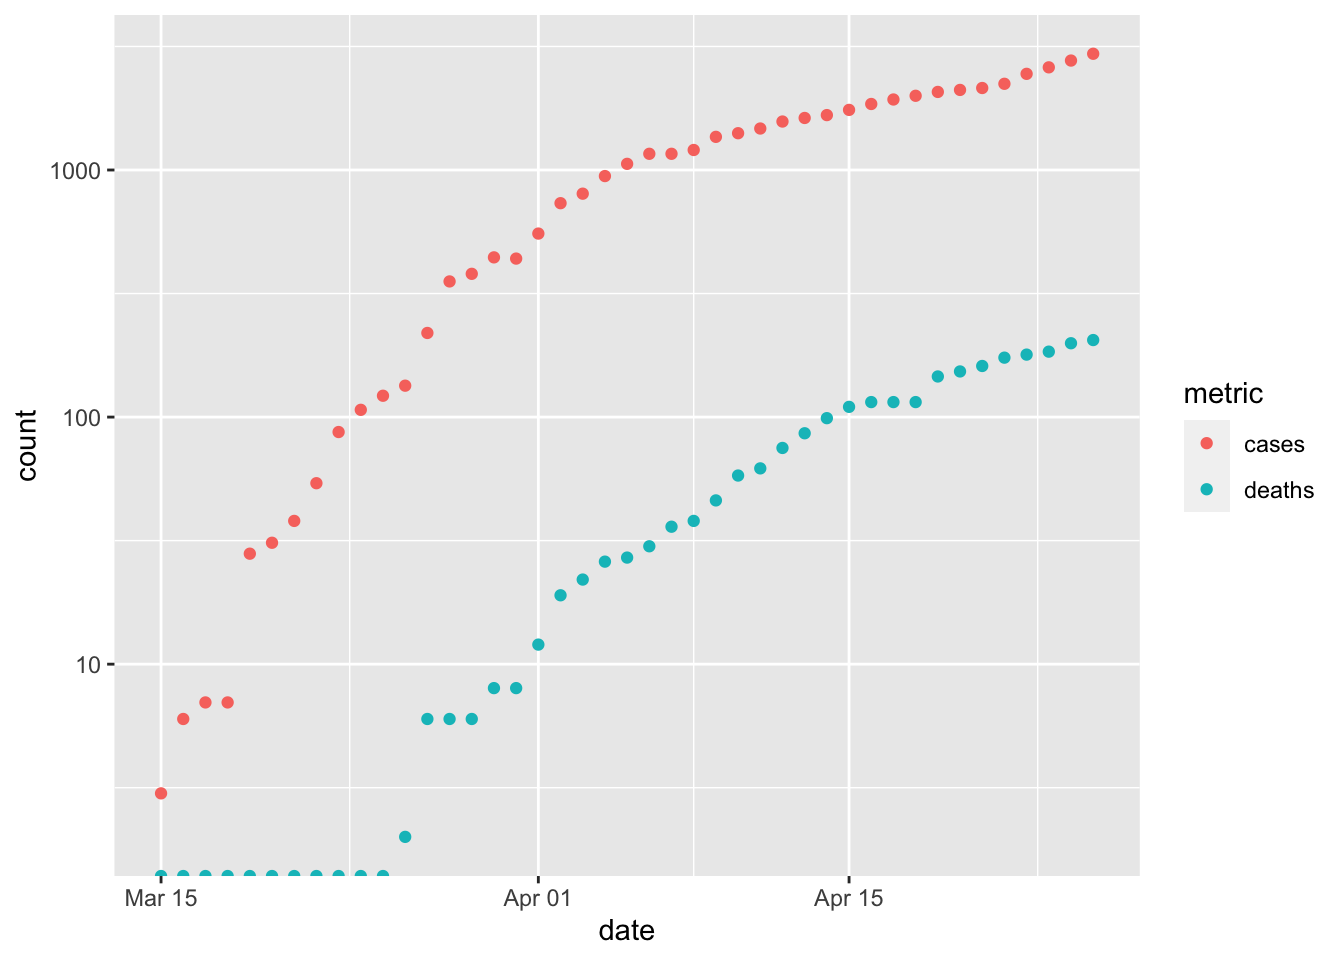
\includegraphics{02-DataFrame_files/figure-latex/unnamed-chunk-43-1.pdf}

  maybe more informative: log-transformed new cases

\begin{Shaded}
\begin{Highlighting}[]
\KeywordTok{plot}\NormalTok{( new_cases }\OperatorTok{~}\StringTok{ }\NormalTok{date, erie, }\DataTypeTok{log =} \StringTok{"y"}\NormalTok{, }\DataTypeTok{main =} \StringTok{"New Cases, Erie County"}\NormalTok{ )}
\CommentTok{## Warning in xy.coords(x, y, xlabel, ylabel, log): 3 y values <= 0 omitted from}
\CommentTok{## logarithmic plot}
\end{Highlighting}
\end{Shaded}

  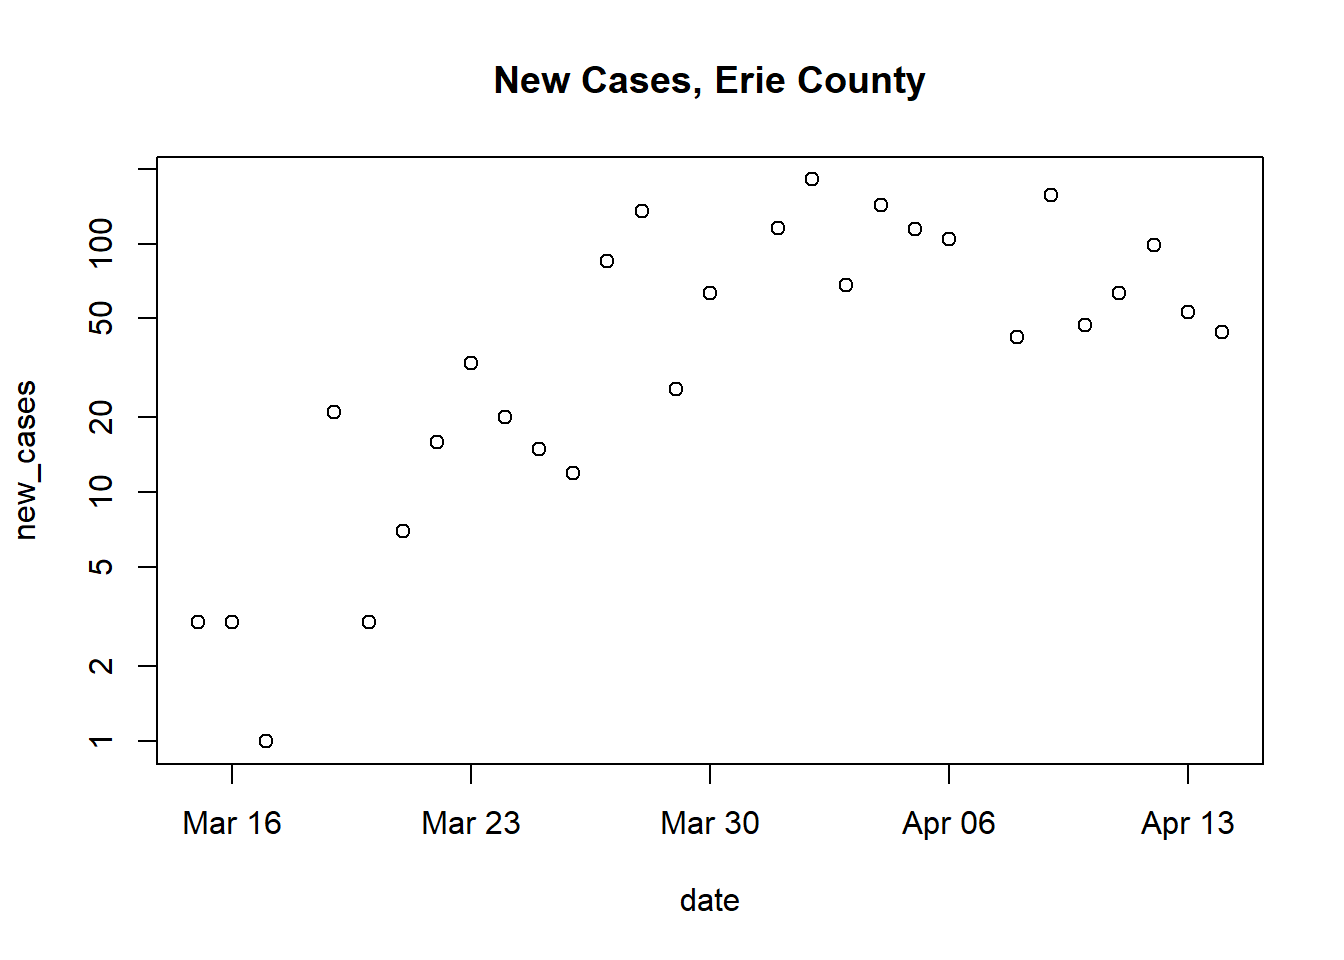
\includegraphics{02-DataFrame_files/figure-latex/unnamed-chunk-44-1.pdf}
\item
  Help: \texttt{?plot.formula}
\end{itemize}

Summary: calculate maximum (total) number of cases per county in New York state

\begin{itemize}
\item
  For Erie county, let's see how to calculate the maximum (total) number of cases

\begin{Shaded}
\begin{Highlighting}[]
\KeywordTok{max}\NormalTok{(erie}\OperatorTok{$}\NormalTok{cases)        }\CommentTok{# one way...}
\CommentTok{## [1] 1668}
\KeywordTok{with}\NormalTok{(erie, }\KeywordTok{max}\NormalTok{(cases)) }\CommentTok{# ... another}
\CommentTok{## [1] 1668}
\end{Highlighting}
\end{Shaded}
\item
  Subset US data to New York state

\begin{Shaded}
\begin{Highlighting}[]
\NormalTok{ny_state <-}\StringTok{ }\KeywordTok{subset}\NormalTok{(us, state }\OperatorTok{==}\StringTok{ "New York"}\NormalTok{)}
\end{Highlighting}
\end{Shaded}
\item
  Summarize each county in the state using \texttt{aggregate()}.

  \begin{itemize}
  \item
    First argument: summarize \texttt{cases} grouped by \texttt{county} -- \texttt{cases\ \textasciitilde{}\ county}
  \item
    Second argument: data source -- \texttt{ny\_state}
  \item
    Third argument: function to apply to each subset -- \texttt{max}

\begin{Shaded}
\begin{Highlighting}[]
\NormalTok{max_cases_by_county <-}\StringTok{ }\KeywordTok{aggregate}\NormalTok{( cases }\OperatorTok{~}\StringTok{ }\NormalTok{county, ny_state, max)}
\KeywordTok{head}\NormalTok{(max_cases_by_county)}
\CommentTok{##        county cases}
\CommentTok{## 1      Albany   535}
\CommentTok{## 2    Allegany    28}
\CommentTok{## 3      Broome   146}
\CommentTok{## 4 Cattaraugus    32}
\CommentTok{## 5      Cayuga    33}
\CommentTok{## 6  Chautauqua    23}
\end{Highlighting}
\end{Shaded}
  \end{itemize}
\item
  \texttt{subset()} to select counties

\begin{Shaded}
\begin{Highlighting}[]
\KeywordTok{subset}\NormalTok{(}
\NormalTok{    max_cases_by_county,}
\NormalTok{    county }\OperatorTok\StringTok{ }\KeywordTok{c}\NormalTok{(}\StringTok{"New York City"}\NormalTok{, }\StringTok{"Westchester"}\NormalTok{, }\StringTok{"Erie"}\NormalTok{)}
\NormalTok{)}
\CommentTok{##           county  cases}
\CommentTok{## 14          Erie   1668}
\CommentTok{## 29 New York City 110465}
\CommentTok{## 57   Westchester  20191}
\end{Highlighting}
\end{Shaded}
\end{itemize}

Summary: calculate maximum (total) number of cases per state

\begin{itemize}
\item
  Use entire data set, \texttt{us}
\item
  \texttt{aggregate()} cases by county \emph{and} state -- \texttt{cases\ \textasciitilde{}\ county\ +\ state}

\begin{Shaded}
\begin{Highlighting}[]
\NormalTok{max_cases_by_county_state <-}
\StringTok{    }\KeywordTok{aggregate}\NormalTok{( cases }\OperatorTok{~}\StringTok{ }\NormalTok{county }\OperatorTok{+}\StringTok{ }\NormalTok{state, us, max )}
\KeywordTok{dim}\NormalTok{(max_cases_by_county_state)}
\CommentTok{## [1] 2737    3}
\KeywordTok{head}\NormalTok{(max_cases_by_county_state)}
\CommentTok{##    county   state cases}
\CommentTok{## 1 Autauga Alabama    23}
\CommentTok{## 2 Baldwin Alabama    87}
\CommentTok{## 3 Barbour Alabama    11}
\CommentTok{## 4    Bibb Alabama    17}
\CommentTok{## 5  Blount Alabama    16}
\CommentTok{## 6 Bullock Alabama     8}
\end{Highlighting}
\end{Shaded}
\item
  \texttt{aggregate()} a second time, using \texttt{max\_cases\_by\_county\_state} and aggregtaing by state

\begin{Shaded}
\begin{Highlighting}[]
\NormalTok{max_cases_by_state <-}
\StringTok{    }\KeywordTok{aggregate}\NormalTok{( cases }\OperatorTok{~}\StringTok{ }\NormalTok{state, max_cases_by_county_state, max )}
\end{Highlighting}
\end{Shaded}
\item
  Explore the data

\begin{Shaded}
\begin{Highlighting}[]
\KeywordTok{head}\NormalTok{(max_cases_by_state)}
\CommentTok{##        state cases}
\CommentTok{## 1    Alabama   620}
\CommentTok{## 2     Alaska   136}
\CommentTok{## 3    Arizona  2056}
\CommentTok{## 4   Arkansas   297}
\CommentTok{## 5 California 10047}
\CommentTok{## 6   Colorado  1402}
\KeywordTok{subset}\NormalTok{(}
\NormalTok{    max_cases_by_state,}
\NormalTok{    state }\OperatorTok\StringTok{ }\KeywordTok{c}\NormalTok{(}\StringTok{"California"}\NormalTok{, }\StringTok{"Illinois"}\NormalTok{, }\StringTok{"New York"}\NormalTok{, }\StringTok{"Washington"}\NormalTok{)}
\NormalTok{)}
\CommentTok{##         state  cases}
\CommentTok{## 5  California  10047}
\CommentTok{## 15   Illinois  16323}
\CommentTok{## 34   New York 110465}
\CommentTok{## 52 Washington   4622}
\end{Highlighting}
\end{Shaded}
\end{itemize}

\hypertarget{day-12-friday-zoom-check-in}{%
\section{Day 12 (Friday) Zoom check-in}\label{day-12-friday-zoom-check-in}}

\hypertarget{day-13}{%
\section{Day 13:}\label{day-13}}

\hypertarget{day-14}{%
\section{Day 14}\label{day-14}}

Self-directed activities.

\hypertarget{three}{%
\chapter{Packages and the `tidyverse'}\label{three}}

\hypertarget{day-15-monday-zoom-check-in}{%
\section{Day 15 (Monday) Zoom check-in}\label{day-15-monday-zoom-check-in}}

\hypertarget{cran}{%
\section{\texorpdfstring{\href{https://cran.r-project.org}{CRAN}}{CRAN}}\label{cran}}

\hypertarget{the-tidyverse-of-packages}{%
\section{\texorpdfstring{The `\href{https://www.tidyverse.org/}{tidyverse}' of packages}{The `tidyverse' of packages}}\label{the-tidyverse-of-packages}}

\hypertarget{day-16}{%
\section{Day 16}\label{day-16}}

\hypertarget{day-17}{%
\section{Day 17}\label{day-17}}

\hypertarget{day-18}{%
\section{Day 18}\label{day-18}}

\hypertarget{day-19-friday-zoom-check-in}{%
\section{Day 19 (Friday) Zoom check-in}\label{day-19-friday-zoom-check-in}}

\hypertarget{review-and-trouble-shoot-25-minutes}{%
\subsection{Review and trouble shoot (25 minutes)}\label{review-and-trouble-shoot-25-minutes}}

\hypertarget{next-week-25-minutes}{%
\subsection{Next week (25 minutes)}\label{next-week-25-minutes}}

\hypertarget{day-20}{%
\section{Day 20}\label{day-20}}

\hypertarget{day-21}{%
\section{Day 21}\label{day-21}}

Self-directed activities.

\hypertarget{four}{%
\chapter{Maps and spatial statistics}\label{four}}

\hypertarget{day-22-monday-zoom-check-in}{%
\section{Day 22 (Monday) Zoom check-in}\label{day-22-monday-zoom-check-in}}

\hypertarget{day-23}{%
\section{Day 23}\label{day-23}}

\hypertarget{day-24}{%
\section{Day 24}\label{day-24}}

\hypertarget{day-25}{%
\section{Day 25}\label{day-25}}

\hypertarget{day-26-friday-zoom-check-in}{%
\section{Day 26 (Friday) Zoom check-in}\label{day-26-friday-zoom-check-in}}

\hypertarget{review-and-trouble-shoot-25-minutes-1}{%
\subsection{Review and trouble shoot (25 minutes)}\label{review-and-trouble-shoot-25-minutes-1}}

\hypertarget{next-week-25-minutes-1}{%
\subsection{Next week (25 minutes)}\label{next-week-25-minutes-1}}

\hypertarget{day-27}{%
\section{Day 27}\label{day-27}}

\hypertarget{day-28}{%
\section{Day 28}\label{day-28}}

Self-directed activities.

\hypertarget{five}{%
\chapter{\texorpdfstring{Bioinformatics with \href{https://bioconductor.org}{Bioconductor}}{Bioinformatics with Bioconductor}}\label{five}}

\hypertarget{day-29-monday-zoom-check-in}{%
\section{Day 29 (Monday) Zoom check-in}\label{day-29-monday-zoom-check-in}}

\hypertarget{day-30}{%
\section{Day 30}\label{day-30}}

\hypertarget{day-31}{%
\section{Day 31}\label{day-31}}

\hypertarget{day-32}{%
\section{Day 32}\label{day-32}}

\hypertarget{day-33-friday-zoom-check-in}{%
\section{Day 33 (Friday) Zoom check-in}\label{day-33-friday-zoom-check-in}}

\hypertarget{review-and-trouble-shoot-25-minutes-2}{%
\subsection{Review and trouble shoot (25 minutes)}\label{review-and-trouble-shoot-25-minutes-2}}

\hypertarget{next-week-25-minutes-2}{%
\subsection{Next week (25 minutes)}\label{next-week-25-minutes-2}}

\hypertarget{day-34}{%
\section{Day 34}\label{day-34}}

\hypertarget{day-35}{%
\section{Day 35}\label{day-35}}

Self-directed activities.

\hypertarget{six}{%
\chapter{Collaboration}\label{six}}

\hypertarget{days-monday-zoom-check-in}{%
\section{5 Days (Monday) Zoom check-in}\label{days-monday-zoom-check-in}}

\hypertarget{days}{%
\section{4 Days}\label{days}}

\hypertarget{days-1}{%
\section{3 Days}\label{days-1}}

\hypertarget{days-2}{%
\section{2 Days}\label{days-2}}

\hypertarget{today-friday-zoom-check-in}{%
\section{Today! (Friday) Zoom check-in}\label{today-friday-zoom-check-in}}

Course review and next steps

\hypertarget{frequently-asked-questions}{%
\chapter*{Frequently asked questions}\label{frequently-asked-questions}}
\addcontentsline{toc}{chapter}{Frequently asked questions}

\begin{enumerate}
\def\labelenumi{\arabic{enumi}.}
\item
  Is the course material available in PDF?

  Yes, click the `Download' icon and PDF format in the title bar of the main document, as illustrated in the figure.

  Remember that the course material is a `work in progress', so the PDF will need to be updated frequently throughout the course. Also, the book is not pretty; that's a task for a separate quarantine!

  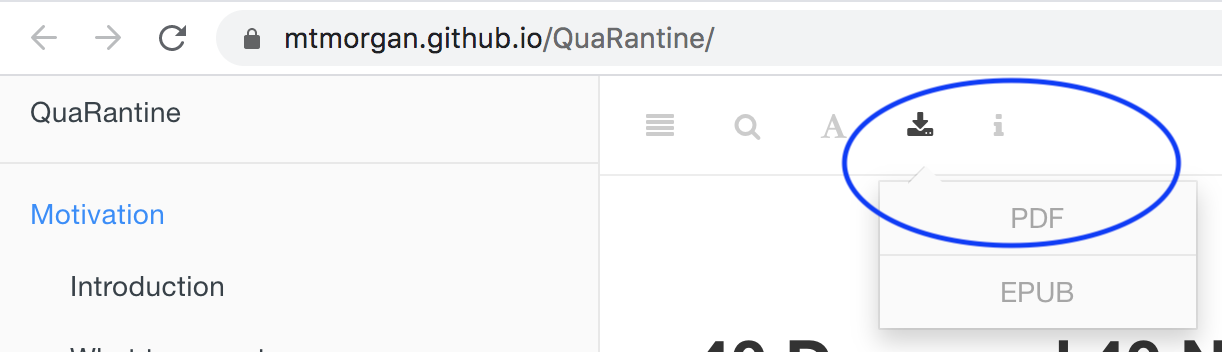
\includegraphics[width=16.97in]{images/99-Download-PDF}
\item
  Whenever I press the `enter' key, the RStudio console keeps saying \texttt{+} and doesn't evaluate my expression! See the figure below.

  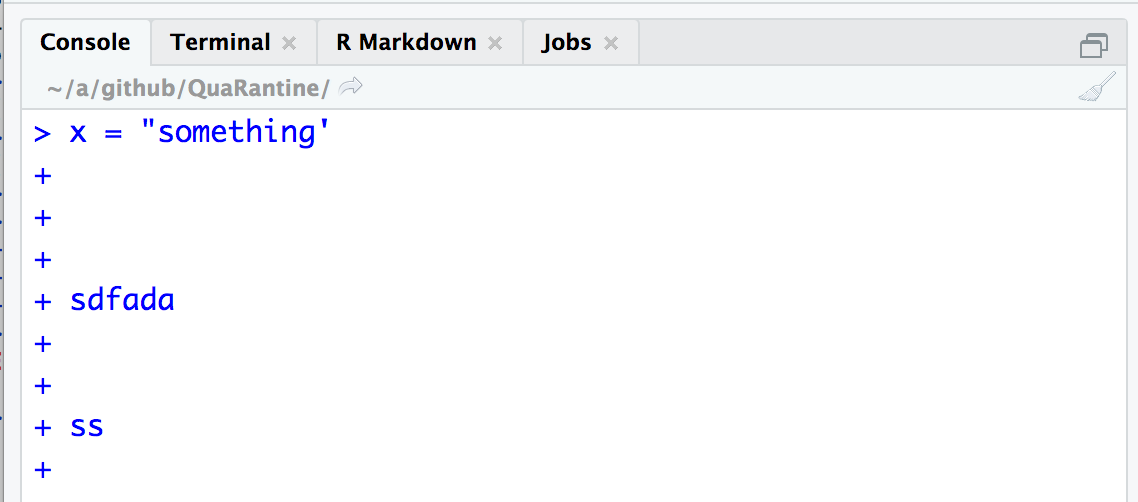
\includegraphics[width=15.81in]{images/99-console-plus-1}

  Notice that you've started a character string with a double \texttt{"}, and tried to terminate it with a single quote \texttt{\textquotesingle{}}. Because the quotes do not match, \emph{R} thinks you're still trying to complete the entry of the variable, and it's letting you know that it is expecting more with the \texttt{+} prompt at the begining of the line.

  A common variant of this is to open more parentheses than you close, as shown in

  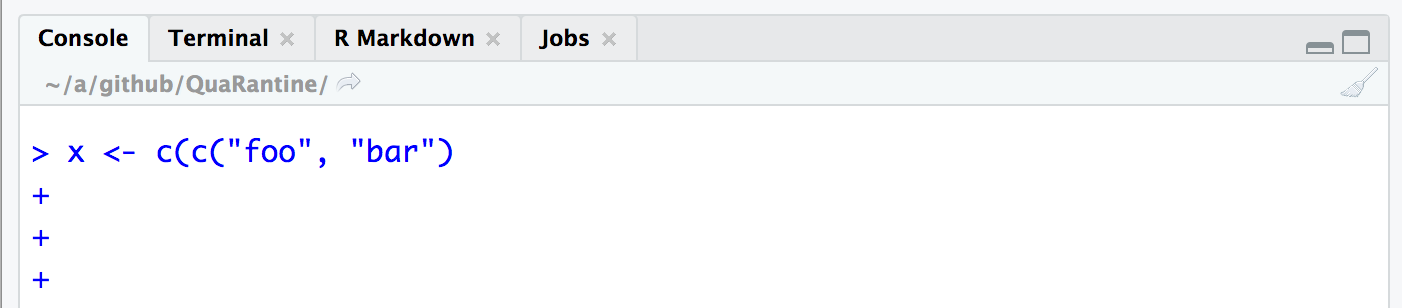
\includegraphics[width=19.47in]{images/99-console-plus-2}

  The solution is either to complete your entry (by entering a \texttt{"} or balancing the parentheses with \texttt{)}) or abandon your attempt by pressing \texttt{control-C} or the escape key (usually in the top left corner of the keyboard)
\end{enumerate}

\bibliography{book.bib,packages.bib}

\end{document}
